\documentclass[12pt]{article}

\usepackage[utf8]{inputenc}
%slippery gypsy packages that need to come first, since others call them after
\usepackage[x11names,dvipsnames,svgnames,table]{xcolor}

% general incantations
\usepackage[export]{adjustbox}
\usepackage{afterpage}
\usepackage{adjustbox}
\usepackage{graphicx}
\usepackage{placeins}
\usepackage{pdfpages}
\usepackage{algorithm2e}
\usepackage{array}
\usepackage{booktabs}
\usepackage[most]{tcolorbox}
\usepackage{calligra}
\usepackage{caption}
\usepackage{datetime}
\usepackage{dblfnote}
\usepackage{dsfont}
\usepackage{etex}
\usepackage{fancyhdr}
\usepackage{fix-cm}
\usepackage{float}
\usepackage[T1]{fontenc}
\usepackage{lipsum}
\usepackage{listings}
\usepackage{transparent}
\usepackage[everyline=true,framemethod=tikz]{mdframed}
\usepackage{mparhack}
\usepackage{multicol}
\usepackage{multirow}
\usepackage{parskip}
\usepackage{lscape}
\usepackage{pdflscape}
\usepackage{pdfpages}
\usepackage{placeins}
\usepackage{rotating}
\usepackage{setspace}
\usepackage{subcaption}
\usepackage{threeparttable}
\usepackage[normalem]{ulem}
\usepackage{verbatim}
\usepackage{soul} %highlighting, strike through etc.

%Line spacing
%\usepackage{setspace}
%\onehalfspacing

%Automated appendices
\usepackage[titletoc,title,header]{appendix} %advanced functionality

%language settings
\usepackage[utf8]{inputenc}
\usepackage[australian]{babel}
\usepackage{csquotes}

%page setup
%this where we adjust the binding offset, if relevant
\usepackage[left=2.5cm,right=2.5cm,top=2.5cm,bottom=2.5cm,headheight=1cm]{geometry}
\usepackage{lastpage} % for page 1 of n footers

%cross referencing
\usepackage[hidelinks]{hyperref}
\usepackage{cleveref}

%maths stuff
\usepackage{amsmath}
\usepackage{mathtools}

\setcounter{secnumdepth}{5}

%lists
\usepackage{enumitem}

%reference list 
\usepackage[backend=biber, style=ieee]{biblatex}
\bibliography{header-footer/ref.bib}
\usepackage{url} %for URL fonts
\urlstyle{same}

% image dir
\graphicspath{ {images/} }

\begin{document}
	\begin{titlepage}
	

\thispagestyle{empty}
\setlength\headheight{0pt} 
\vspace*{1cm}
\begin{center}
\begin{center}
\includegraphics[width=0.5\linewidth]{anu-logo.jpg}            
\end{center}	

\vspace{2cm}

{\Large\bfseries Design of a Low Cost Vector Network Analyser\par}

\vspace{2cm}
{\Large Josh Johnson \par}
u6044123\par

\vspace{1.5cm}
Supervised by\par
Dr. Gerard Borg \\
\vspace{1.5cm}
\large
October 2019


\vspace{4cm}
\small{ A thesis submitted in part fulfilment of the degree of Bachelor of Engineering \par
College of Engineering and Computer Science \par
Australian National University }

\end{center}

\clearpage
\restoregeometry
\end{titlepage}
	\pagenumbering{gobble} 
	\thispagestyle{empty}
\newpage
\vspace*{4cm}
This thesis contains no material which has been accepted for the award of any other degree or diploma in any university. To the best of the author's knowledge, it contains no material previously published or written by another person, except where due reference is made in the text. \par
\vspace{4cm}
Josh Johnson \par
\today
	\pagenumbering{roman}
	\setcounter{page}{0}
	\newpage
	
	\section*{Abstract}
	A vector network analyser capable of measuring S\textsubscript{11} and S\textsubscript{21} over a 25 – 1250 MHz frequency span was designed, assembled, and calibrated. Through comparison against commercially available solutions, it is shown that there are a number of issues with the measured waveforms, which impact the accuracy of magnitude measurements, along with causing significant issues with phase measurements. The design decisions causing these errors are identified, and suggestions are made to resolve them such that a second revision of the design would likely result in a VNA which meets the design specifications. 

	\pagebreak
	
	\tableofcontents
	\pagebreak
	
	\listoffigures
	\pagebreak
	\listoftables
	\pagebreak
	\section*{Glossary}
	\textbf{ADC} - Analog to Digital Converter.

\textbf{ASIC} - Application Specific Integrated Circuit.

\textbf{COTS} - Commercial Off-The-Shelf.

\textbf{dB} - Decibel.

\textbf{dBm} - Decibel power ratio with reference to 1 mW.

\textbf{DDS} - Direct Digital Synthesis. 

\textbf{DSP} - Digital Signal Processing.

\textbf{DUT} - Device Under Test. With reference to a VNA, the device connected to VNA's ports being measured. 

\textbf{ENOB} - Effective Number of Bits.

\textbf{FPGA} - Field Programmable Gate Array.

\textbf{HAL} - Hardware Abstraction Library.

\textbf{ISM} - Industrial Scientific Medical.

\textbf{IP3} - Third Order Intermodulation Product.

\textbf{I/Q} - In-phase / Quadrature. Used in DSP to represent two sinusoids which are 90 degrees out of phase. 

\textbf{LO} - Local Oscillator. 

\textbf{P1dB} - 1 dB Compression Point. 

\textbf{PA} - Power Amplifier.

\textbf{PCB} - Printed Circuit Board. 

\textbf{PCBA} - Printed Circuit Board Assembly.

\textbf{PLL} - Phase Locked Loop.

\textbf{RF} - Radio Frequency.

\textbf{RFIC} - Radio Frequency Integrated Circuit

\textbf{S-parameters} - Scattering Parameters. Elements of a scattering matrix which describe the behaviour of linear electrical networks. 

\textbf{S\textsubscript{MN}} - S-paramater describing the relationship between ports M and N in an electrical system. Common s-parameters are S\textsubscript{11} which represents the reflected power incident on port one, and S\textsubscript{21}, which represents the gain of a DUT between ports 2 and 1. 

\textbf{SMT} - Surface Mount Technology.

\textbf{SPDT} - Single Pole Double Throw switch. 

\textbf{SP4T} - Single Pole 4 Throw switch. 

\textbf{VCO} - Voltage Controlled Oscillator.

\textbf{VNA} - Vector Network Analyser. Electronic test and measurement instrument which measures s-parameters of electrical networks. 

\textbf{VSWR} - Voltage Standing Wave Ratio

	\pagebreak
	
	\pagenumbering{arabic}
	\section{Introduction}
	\label{sec:intro}
	\subsection{Background}
A Vector Network Analyser is a radio frequency test and measurement instrument which measures the S-parameters of a device under test. VNAs are used extensively in the design of RF devices as they allow the gain and phase response of RF components such as antennas, filters, amplifiers, and mixers to be characterised over the their operating frequencies, which is crucial for successful design and manufacturing of RF devices.

Vector network analysers work by generating a reference frequency which is passed into a device under test (DUT), and through comparing the incident and reflected RF signals from ports of the DUT the change in waveform caused by the DUT can be determined. Through sweeping the frequency, the response at each port of the VNA can be determined over a frequency range, and through signal processing the gain and phase response of each port of the DUT can be determined. From this data, S-paramater, VSWR, along with Smith chart and polar plots are able to be generated, which allows analysis of the DUT along with informed decisions regarding the function of the DUT to be made, which is required for the engineering of modern devices. 

Given that VNAs are intricate pieces of engineering and are sold in low volume to engineering firms, their price represents this high level of performance and niche market, with VNAs typically ranging from tens of thousands to millions of dollars. Given this pricing is prohibitively expensive for teaching in educational institutions and far more than most electronics hobbyists have to spend, this limits the scope of projects and learning experiences which can be accessed outside of professional engineering environments. 

\subsection{Aim}
The aim of this thesis is design and build a VNA which is significantly cheaper than the commercial offerings, as this will lower the barrier of entry to RF engineering and enable more hobbyists and educators to build or purchase a VNA which fits their needs. Whilst this VNA will not have the frequency and dynamic range, accuracy, UI, or speed of a commercial VNA, it will still be able to provide indicative measurements which are sufficiently accurate for home or educational use, along with providing an interesting learning exercise in the areas of radio frequency and embedded engineering.  

\newpage
\subsection{Previous Work}
Numerous people have attempted to make their own VNAs with varying specifications and architectures, and the work outlined in this thesis has been heavily inspired by many of these projects. 

Henrik Forsten has designed two VNAs, both of which cost less than \$1000 and operate upto 6 GHz. His first design \cite{henrik_1} utilised printed microstrip couplers to couple the RF, along with a microcontroller with a 12 bit ADC sampling at 10 MSPS to sample downconverted RF. This design worked, however due to port to port leakage, variances with coupling over the frequency range, and slow processing due to the microcontroller struggling to keep up with the ADC sampling speed required, it did not function well enough for day to day use.  

Forsten's second design \cite{henrik_2} replaced the microcontroller with an FPGA and external 14 bit, 40 MSPS ADC, which allowed both data capture and signal processing to be completed in real time. He also designed resistive bridge couplers which had significantly better performance over the operating frequency range, and whilst this design preformed significantly better, the extra components resulted in an increased BOM and the couplers took up significant space. He did however show that a feature complete VNA could be manufactured for significantly less than commercial offerings, using processes and components which can be easily acquired by hobbyists.  

Other architectures have utilised a dedicated RFIC in the form of Analog Devices' AD8302 gain and phase detector, which handles all of the gain and phase detection in silicon, and allows for low frequency sampling of two analogue outputs to determine gain and phase. This results in a significant decrease in signal processing required, allowing for lower cost embedded processors being utilised in the design. 

One such design \cite{nagy_vna} utilised an AD8302 and COTS components in the form of development boards to prototype a VNA. That project showed that an AD8302 based VNA was practicable, however due to the use of development board for each functional block the cost came out to roughly \$2000, significantly higher than the target for this project. The design also ran into issues regarding zero crossings of phase due to long conformance errors in the AD8302, however it was noted that this is likely correctable with sufficient signal processing.  

Another design based around the AD8302 \cite{torre_vna} utilised a direct digital synthesis IC with I and Q outputs to feed two AD8302 ICs, which enabled them to work around the zero crossing issue outlined above. However, due to the inherit limitations of DDS architecture, they were limited to 5 - 80 MHz, significantly less than the bandwidth of most VNAs. 

\subsection{Overview}
An overview of the sections within this thesis is outlined below.

\textbf{Chapter 2 - Requirements, Constraints, and Specifications} details the requirements and constraints of the VNA, and will enable the design scope and device specifications to be determined. 

\textbf{Chapter 3 - Design} covers design of the VNA. Resulting from theory of operation and research of other low cost VNAs, the high level architecture along with detailed design was undergone and though testing candidate components were validated and selected.  

\textbf{Chapter 4 - Implementation and Assembly} details printed circuit board layout along with assembly of the PCB. Furthermore, mechanical design of an enclosure along with firmware and software implementation is discussed. 

\textbf{Chapter 5 - Testing and Conclusion} covers a comparison of measurements to commercial VNAs, along with a discussion of the results and proposes future avenues for improvement of the VNA. 
	
	\section{Requirements, Constraints and Specifications}
	\label{sec:requirements}
	\subsection{Requirements}
\label{subsec:requirements}
To be useful the VNA must be able to measure the gain and phase response of a DUT over a given frequency range, and have industry standard features including plotting and file handling which would allow it to replace a commercial VNA in certain situations. 

\subsection{Constraints}
\label{subsec:contraints}
There are a number of constraints acting upon the project which will constrain the design and function of the device. The desire of the project is to build the most performant VNA that can be designed within the below constraints. 

\begin{itemize}
	\item \textbf{Cost -} as outlined in the introduction, the major goal of this project is to build a VNA at a significantly lower price than commercial offerings. As such, there will be a large number of trade-offs required to bring the price down, and as a result the accuracy, dynamic range, bandwidth, and numerous other performance characteristics will be traded off in an attempt to reach the desired price point.
	\item \textbf{Component Selection -} in an attempt to decrease the cost of low volume manufacture, along with the engineering time and resources required, all components in the design must be commercial off-the-shelf, as this will reduce the cost and time required during development and manufacturing. 
	\item \textbf{Resources -} due to a number of factors including skill level of the designer, limited time frame, monetary resources available, and the lack to access to test gear and industry specific tools such as Keysight's Advanced Design System and CST Microwave Studio, the complexity of the project needs to be limited to ensure that a minimum viable product is able to be produced within the given time frame.   
\end{itemize}

\subsection{Specifications}
\label{subsec:specifications}
Taking the above outlined requirements and constraints into consideration, specifications for the VNA can be determined. Given that there are no hard numbers specified, and that the goal for the VNA is one which is as performant and feature complete as possible given the constraints, many of the exact specifications of the VNA will be determined during the design process. This allows cost to be a key factor during the architecture design and component selection, as small decreases in performance are able to be made to save significant cost, which would not be possible if the system requirements were highly specified. In saying this, there are some key minimum specifications and high level architectural choices which will help narrow the design scope:
\begin{itemize}
	\item \textbf{Bandwidth -} the VNA should have at least 1GHz of bandwidth, as this will allow both the 433MHz and 915 MHz ISM bands to be within the frequency span, and as such enable testing of components which can be utilised without an amateur radio licence. 
	\item \textbf{Interface -} controlling the VNA from a computer will not only remove the need for a display on device which will lower cost, but also significantly reduce the embedded compute power required whilst allowing for use of tools such as Python's NumPy and scikit-rf for data processing and VNA calibration, along with Qt and Matplotlib to provide a user interface with a much lower time investment than developing the required functionality from scratch on embedded hardware. 
	\item \textbf{Ports -} whilst most modern VNAs allow for all S-parameters of a DUT to be measured, this requires extra hardware for the routing of signals around the board which drives up cost and complexity. Given that the majority of measurements only involve S\textsubscript{11} and S\textsubscript{21}, through only measuring these two parameters the complexity and cost of the VNA can be reduced whilst not significantly impeding function of the device. If S\textsubscript{22}, S\textsubscript{12}, or a DUT with more than two ports is required to be measured, external connections to the DUT can be altered to allow these measurements to take place.  
	\item \textbf{Licencing -} the VNA should be able to be designed, manufactured, programmed, and operated using solely free tools, and where practicable open source tools. This ensures the VNA is able to be operated without any expenses other than the cost of hardware, whilst also ensuring that the hardware, firmware, and software is able to be viewed and modified by anyone without having to purchase proprietary tools, which may be prohibitively expensive and become obsolete, preventing access to the source files used during design. 
\end{itemize}
	\pagebreak
	
	\section{Design}
	\label{sec:design}
	Design of the VNA takes place in two steps: high level architectural design where the functional blocks of the system are determined, followed by detailed design where specific components are chosen to meet the needs of each functional block. 

\subsection{Architecture}
\label{subsec:architecture}
A VNA has four main functional blocks as shown in Figure \ref{fig:keysight_vna_block_diag}: source for stimulus, signal separation, receiving / detecting, and processing / display. Each of these functional blocks plays a key role in the function of a VNA and will be discussed below.
\begin{figure}[H]
	\centering
	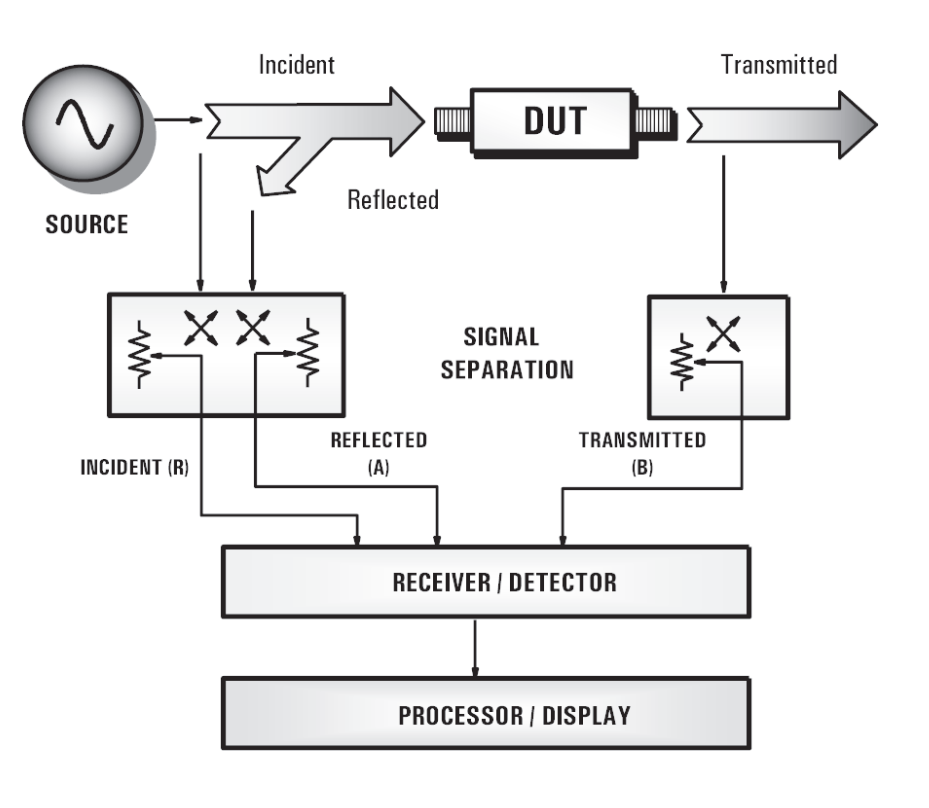
\includegraphics[width=0.6\linewidth]{keysight_vna_block_diag.PNG}
	\caption{Generalised Network Analyser Block Diagram \cite{keysight_vna_basics}}
	\label{fig:keysight_vna_block_diag}
\end{figure}

\subsubsection{Signal Source}
\label{subsec:signal source}
The signal source is the first functional block in the signal path of a VNA, and is responsible for providing the stimulus used for the test system. This source is typically swept over frequency, but can also be swept over power to measure the required parameters. Two primary considerations for the signal source are the phase noise of the signal, which can cause issues with narrow bandwidth measurement if it is too large, and the spectral purity of the signal, which can result in incorrect frequency response measurements if there are spurious tones or harmonics in the output spectrum. 

Typically the signal sources utilise a voltage controller oscillator, which is able to generate continuous wave signals over a wide bandwidth through the use of a PLL to multiply a reference clock to the required frequency. Single chip solutions are available which contain a PLL and multiple VCOs to enable a wide frequency range with only a few external passives, and whilst these PLLs are easy to implement and control, they typically have increased phase noise, harmonics, and spurs compared to a PLL which uses multiple discrete components to close the loop, which is seen on higher end devices where the quality of the output spectrum is key. 

To allow control over the output power level, a power amplifier, programmable attenuator, and power detector can be utilised to provide closed loop control over the output power level. Key features of the source levelling components are that they can provide the required power level over the frequency range being swept, along with not distorting the signal being output by the source. 

\subsubsection{Signal Separation}
\label{subsubsec:signal seperation}
Signal separation is the next functional block in the system, and is utilised to measure a portion of the source for analysis in the receiver / detector subsystem. They are used to measure both the power being output by the source, along with the incident and reflected waves at connections to the DUT. The latter two measurements require directional couplers, as both the incident and reflected waves are on the same PCB trace whilst travelling in opposing directions, and as such high directivity is required to ensure that only the signal travelling in the desired direction is being measured. 

The three most common methods for coupling signals are resistive dividers, which are broadband but lack directivity and have high loss, directional couplers, which have low loss however their coupling and directivity are limited in bandwidth, and directional bridges, which are broadband, can have high directivity, and have lower loss than restive dividers. 

\subsubsection{Receiver / Detector}
\label{subsubsec: receiver detector}
Most vector network analysers utilise a tuned narrowband detector where the RF incident upon the DUT is downconverted to an intermediate frequency, with an ADC sampling the signal and digital signal processing is then preformed to determine the gain and phase of the IF signal. This design results in high sensitivity and dynamic range, along with good harmonic and spurious tone rejection, and a significantly lower noise floor than other methods. However due to the high sample rates of the ADC required to meet the Nyquist sampling frequency of the signal, this method requires a fast sampling ADC, and the corresponding amount of computing power to preform the signal processing to determine the amplitude and phase of the signal, which is comparatively expensive to other methods.  

In scalar network analysers, diode based detectors are often used as they provide a cost effective solution to measuring power. However they are broadband which can result in spurious measurements at unintended frequencies, do not have the sensitivity and dynamic range of a tuned detector, and are only able to measure gain, not phase of a signal. As such they are not suitable for use in a vector network analyser where phase measurements are required.

A third potential receiver utilises the AD8302 from Analog Devices, which is a RF / IF Gain and Phase Detector.\cite{ad8302_datasheet} The AD8302 contains dual demodulating log amplifiers and a phase detector, which generates two analog  voltages which correspond to the gain and phase difference between the input RF signals. This design has the same issues as a diode detector due to utilising diode detectors internally for gain detection, however it resolves the phase measurement issue due to generating phase difference as a second output. There are however some signal processing challenges which need to be overcome with the phase detection, as the output can not differentiate between positive and negative phase, and also has significant log conformance error at small phase differences and higher frequencies. However, given that its cost is between the two other solutions outlined above, it may be a cost effective solution to gain and phase detection if high dynamic range is not required. 

\subsubsection{Processor / Display}
\label{subsubsec:processor display}
The final functional block in a VNA is the processing and display of the received data, where the raw data measured by the receiver is transformed and displayed in various ways which enable the user to make informed decisions about the measurements being taken. 

Depending on the amount of processing required, the compute requirements may vary from multiple custom ASICs for the digital signal processing combined with a Windows install, touch screen, and physical buttons for the application layer, all the way through to a Cortex M0 microcontroller with a small TFT display which handles both the signal processing and display to the user. In recent years, companies such as Tektronix have been rolling out 'headless' devices which utilise the user's computer to handle the application layer, enabling smaller and cheaper test and measurements devices as they no longer require a screen along with the user interface on device. 

\subsubsection{Chosen Architecture} 
\label{subsubsec:chosen architecture}
Taking into account the constraints and specifications in combination with the common architectures outlined above, the desired architecture for the device can be decided so that the scope can be narrowed for detailed design. 
\begin{itemize}
	\item \textbf{Signal Source -} a single chip PLL with integrated VCO would be well suited for the VNA, as the benefits from a single chip solution which is cheaper, takes up less board space, and is easier to configure than a PLL made of discrete components far outweighs the loss of performance which will result the single chip solution. 
	\item \textbf{Signal Separation -} whilst a directional bridge would be ideal as it has high directivity whilst working over a wide frequency range, the desire for all components to be COTS rules this out, as they are typically designed into the PCB and as such would require extensive simulation and testing, even if a reference design such as the work of of N. Drobotun and P. Mikheev in their paper "A 300khz-13.5ghz directional bridge" \cite{resistive_coupler} was to be implemented. As such a directional coupler will be the best option, with the main limitation being the availability of broadband directional couplers in the desired frequency range. 
	\item \textbf{Receiver / Detector -} whilst a tuned narrowband detector would be ideal, the cost of a high sample rate ADC along with a FPGA to do the signal processing would exceed the desired BOM of the VNA. As such, the AD8302 from Analog Devices will form the receiver as it has sufficient performance characteristics whilst being significantly cheaper than a digital front end. 
	\item \textbf{Processor / Display -} given the use of an AD8302 for gain and phase detection, a microcontroller will have sufficient processing power and can be utilised to keep costs low. Furthermore, offloading data processing and visualisation to a host computer will allow for further reduction in cost due to not requiring the extra processing power, display, or user interface controls to be added to the device.
\end{itemize}

\subsection{Detailed Design}
\label{subsec:detailed_design}
With the architecture of the VNA outlined and constraints which influence component selection documented, detailed design of the VNA can begin. The following section outlines key considerations in component choice, low level design details, along with some of the testing and characterisation which was done prior to finalising the first schematic. A block diagram of the system can be found in Figure \ref{fig:vna_block_diag}, with the full schematic for the VNA in Appendix \ref{appen:vna_design_files}.

\subsubsection{LO Generation}
The first part of the RF chain begins with the LO, as it generates the signal used throughout the VNA. As outlined in the architecture section, a single chip solution is desired and resulting from research two primary options were found: ADF4351 from Analog Devices, and the MAX2871 from Maxim. The Table \ref{table:lo_comparison} summaries their specifications. 

\begin{landscape}
	\begin{figure}
		\centering
		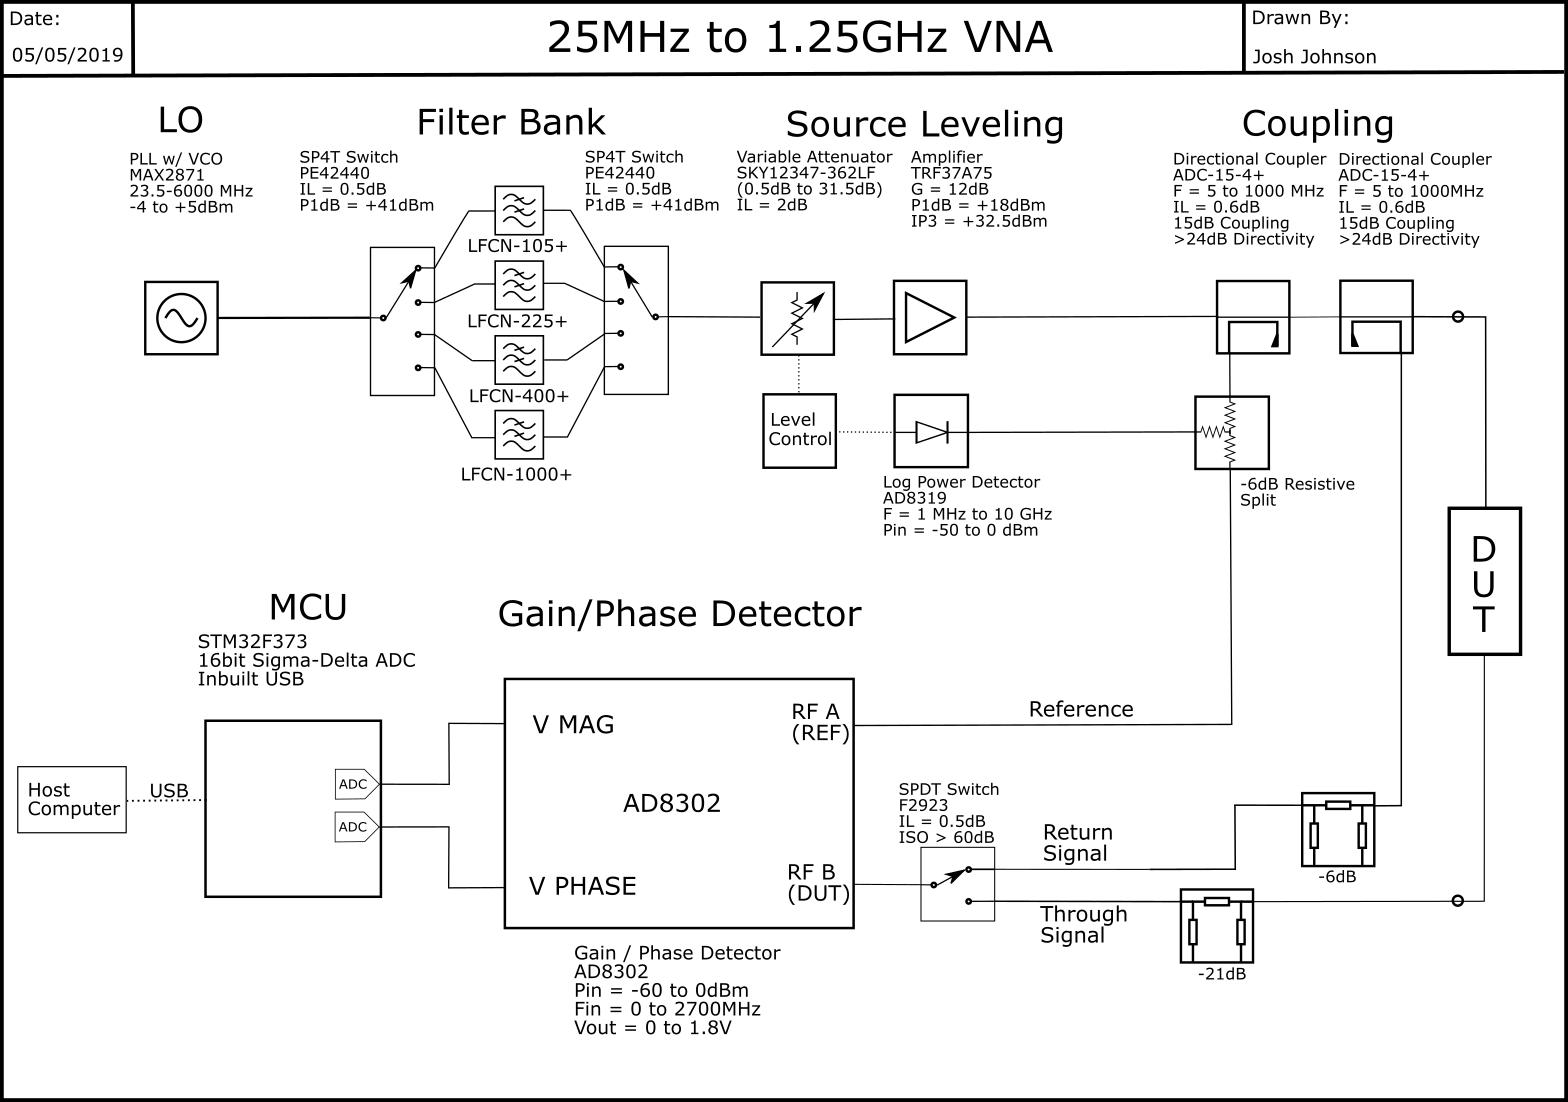
\includegraphics[width=\linewidth]{josh_block_diag.png}
		\caption{Functional Block Diagram of the VNA}
		\label{fig:vna_block_diag}
	\end{figure}
\end{landscape}

\begin{table}[H]
	\caption{Comparison of LO generation ICs}
	\label{table:lo_comparison}
	\centering
\begin{tabular}{|c|c|c|}
	\hline
	\multicolumn{1}{|l|}{}          & \textbf{MAX2871} & \textbf{ADF4351} \\ \hline
	\textbf{Frequency Range MHz}    & 23.5 - 6000      & 35 - 4400        \\ \hline
	\textbf{Fractional / Integer N} & Fractional       & Fractional       \\ \hline
	\textbf{Max Output Power (dBm)}   & 5                & 5                \\ \hline
	\textbf{Cost (\$ at Quantity 1)}& 17               & 23             \\ \hline
	\textbf{Example Code}           & No               & Yes              \\ \hline
\end{tabular}
\end{table}
\vspace{-1em}
As can be seen from Table \ref{table:lo_comparison}, the MAX2871 has a wider frequency range, whilst having a lower cost and having the same maximum output power and Fractional-N PLL as the AD4351. The only downside of it for our application is that there is no example code provided by Maxim, and this combined with it's poor data sheet may result in extended firmware development time, whereas Analog Devices provides example code along with an extremely well documented data sheet and application notes. Given there is no cost associated with firmware development and that the goal for the device is to have the widest frequency band at the lowest cost possible, the MAX2871 was chosen due to it's superior specifications. 

\subsubsection{LO Filtering}
\label{subsubsec:lo filtering}
Due to the LO utilising a divided down output for frequencies below 3 GHz, there are significant harmonics in the output signal which need to be filtered out. As will be discussed later, the directional couplers chosen operate up to 1 GHz, and as such filters need to be chosen which operate up to this frequency. Four filters from Mini-Circuits's LFCN series were chosen, with the goal of only frequencies below the second harmonic of a signal being able to pass through, as this would remove most of the unwanted harmonics. In an ideal world this would prevent all harmonics from a fundamental greater than 50 MHz from passing through the RF chain,  however due to the roll off of the filter, along with some poor decisions resulting from not paying enough attention to the data sheets and not fully understanding of the importance of an harmonic free output, the filter selection resulted in issues which will be discussed in \S \ref{sec:implementation}. The chosen filters are tabulated below, along with the frequencies at which 1, 3, and 40 dB of attenuation are measured. 

\begin{table}[H]
	\caption{Selected Filters}
	\label{table:selected_filters}
	\centering
	\begin{tabular}{|c|c|c|c|c|}
		\hline
		\textbf{}               & \textbf{LFCN-105+} & \textbf{LFCN-225+} & \textbf{LFCN-400+} & \textbf{LFCN-1000+} \\ \hline
		\textbf{1 dB IL (MHz)}  & 125                & 250                & 410                & 1100                \\ \hline
		\textbf{3 dB IL (MHz)}  & 180                & 350                & 560                & 1300                \\ \hline
		\textbf{40 dB IL (MHz)} & 265                & 510                & 680                & 1800                \\ \hline
	\end{tabular}
\end{table}
\vspace{-1em}
During the design of the VNA, filters were chosen based off their 1 dB attenuation, as that is the headline figure which Mini-Circuits names their products by. At the time the filter choices were being made, it was unknown that the PLL's output below 3 GHz was divided down, and the significant amount of harmonics this would result from the output waveform being a square wave instead of a sinusoid. In hindsight, now knowing the importance of harmonics being attenuated by more than the $\sim$ 35 dB of dynamic range of the VNA, filters would be chosen based upon their frequency at which 40 dB of insertion loss is measured, as shown by the bottom row of Table \ref{table:selected_filters}. 

For the filters to be switched in and out of the signal path, two SP4T switches capable of functioning down to 25 MHz were required. The PE42440 from pSemi was chosen due to their flat insertion loss across the frequency band of interest, along with low price. 

\subsubsection{LO Levelling}
With the hardware described above a signal can be generated over a broad frequency range, however other than the 3 dB steps programmable from the MAX2871, there is no control over the output power. A flat power profile is required as a DUTs performance may vary as a function of power, and as such being able to keep the output power at a constant value is crucial. This is implemented through the use of a programmable attenuator and power amplifier to set a given output power, and a logarithmic power detector and firmware to measure and provide closed loop control over the output power. 

With the desired programmable attenuator having a flat insertion loss from 25 MHz to 1 GHz and fine power control, the PE43711 from pSemi was chosen as it allowed for 0.25 dB attenuation steps up to 31.75 dB whilst having a flat frequency response throughout. A HMC313 from Hittite was chosen as the PA, once again due to it's flat frequency response across the operating frequencies. Finally, an AD8319 log power detector was chosen to provide the power sensing, as it's logarithmic output would allow for easy measurement of the logarithmic RF power from an analog pin on the host microcontroller. 

A test board was designed with the above components interfacing with an external microcontroller to implement the control algorithm, and through testing was shown to work. However, during testing it was noticed that at power levels above 0 dBm there were significant harmonics in the spectrum, and due to this varying with power it was identified that the issue was non-linearities in the amplifier causing the unwanted tones. As such a new test board based around the TRF37A75 from Texas Instruments was designed, and through testing it was shown that the higher P1dB and IP3 was sufficient for the power levels required for the source levelling block. One downside of the TRF37A75 is that the gain drops off steeply below 40 MHz, however due to the programmable attenuator being situated in series with the PA this can be compensated for by decreasing the attenuation at the lower frequencies. The key differences between the HMC313 and TRF37A75 are highlighted in Table \ref{table:power_amps}.

\begin{table}[H]
	\caption{Comparison of Power Amplifiers}
	\label{table:power_amps}
	\centering
\begin{tabular}{|c|c|c|}
	\hline
	\multicolumn{1}{|l|}{}           & \textbf{HMC313} & \textbf{TRF37A75} \\ \hline
	\textbf{Frequency Range (MHz)}   & DC - 6000       & 40 - 6000         \\ \hline
	\textbf{Gain (dB)}               & 17              & 12                \\ \hline
	\textbf{P1dB (dBm)}              & 14              & 18                \\ \hline
	\textbf{IP3 (dBm)}               & 27              & 32.5              \\ \hline
	\textbf{Current Draw (mA at 5V)} & 50              & 80                \\ \hline
	\textbf{Cost (\$ at Quantity 1)} & 6               & 2.5               \\ \hline
\end{tabular}
\end{table}
\vspace{-1em}
\subsubsection{Directional Couplers}
Directional couplers are one of the key components in a VNA, as they set the frequency and dynamic range of the device. A wide frequency range, flat coupling, high directivity, along with low insertion and return loss are all key measurements which play a role in determining the performance of the instrument. Whilst it would have been preferable to design a resistive directional bridge which has superior characteristics for the above parameters, due to the desire for solely COTS products to be utilised the ADC-15-4+ from Mini-Circuits is the best fit, and it's key features are outlined in Table \ref{table:coupler}. 
\begin{table}[H]
	\caption{Key Parameters of the ADC-15-4+ Directional Coupler}
	\label{table:coupler}
	\centering
\begin{tabular}{|c|c|}
	\hline
	\multicolumn{1}{|l|}{}         & \textbf{ADC-15-4+} \\ \hline
	\textbf{Frequency Range (MHz)} & 5 - 1000           \\ \hline
	\textbf{Insertion Loss (dB)}   & 0.4 - 0.8          \\ \hline
	\textbf{Coupling (dB)}         & 15                 \\ \hline
	\textbf{Directivity (dB)}      & 24 - 35            \\ \hline
	\textbf{Return Loss (dB)}      & \textgreater 25    \\ \hline
\end{tabular}
\end{table}
\vspace{-1em}
During qualification of the ADC-15-4+, the directivity was measured out to 2000 MHz and it was noted that whilst it decreased after 1000 MHz, directivity stayed above 24 dB until 1300 MHz, and coupling was also flat out to that frequency. As such the operational range of the coupler can be increased to 5 - 1300 MHz for our use in the VNA. 

\subsubsection{Gain and Phase Detection}
With the AD8302 by Analog Devices being chosen for gain and phase detection, there is little design work do be done due to reference designs being available. However there are a few challenges which need to be overcome to successfully transform it's outputs to gain and phase values, and understanding these will be key to selecting the correct processor to sample and process the information. Figure \ref{fig:ad8302_block_diag} highlights the Functional Block Diagram of the AD8302 which may assist with understanding the function of the device. 

\begin{figure}[H]
	\centering
	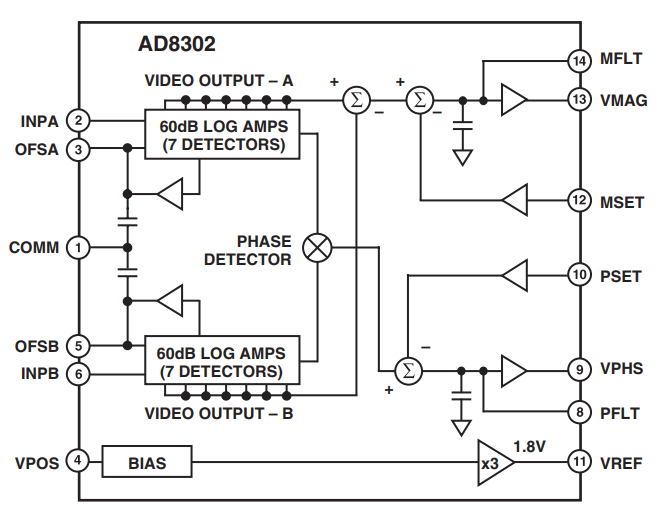
\includegraphics[width=0.8\linewidth]{ad8302_blockdiagram.png}
	\caption{Functional Block Diagram of AD8302}
	\label{fig:ad8302_block_diag}
\end{figure}

Given RF inputs on INPA and INPB, the AD8302 outputs two analog signals ranging from 0 to 1.8V on VMAG and VPHS which correspond to the gain and phase difference between the two RF signals. However these outputs are not perfect, and as such there are various considerations which need to be taken into account to ensure that the gain and phase differences are represented accurately. 

\textbf{VMAG Log Conformance Error} \\
The VMAG output of the AD8302 shown in Figure \ref{fig:ad8302_VMAG_conformance}, which represents the magnitude ratio of the two RF inputs, has decreased linearity towards the ends of its span. Although this could be compensated for through using a non linear model for the voltage to gain conversion, given that the error exceeds 0.5 dB at $\pm$27 dB, which is not only enough dynamic range for many measurements but only 3 dB from the limits of the output, it will not be compensated for due to the limited time available for this project.  
\begin{figure}[H]
	\centering
	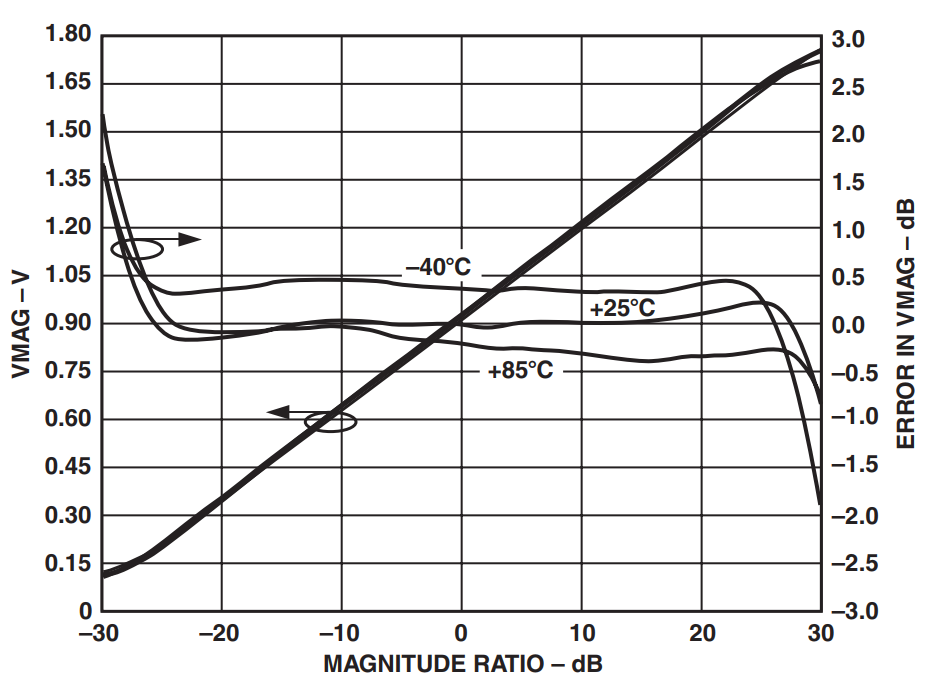
\includegraphics[width=0.6\linewidth]{ad8302_gain_conformance_error.png}
	\caption{VMAG Log Conformance Error}
	\label{fig:ad8302_VMAG_conformance}
\end{figure}

\textbf{VPHS Sign Ambiguity} \\
As shown in Figure \ref{fig:ad8302_VPHS_frequency}, the output voltage representing the phase difference is unable to differentiate between positive and negative phase, due to the output voltage being symmetrical around zero phase difference. It should however be noted that the gradient between -180 and 0 phase is different to 0 to +180 degrees, and as such by looking at how the phase changes as a function of frequency the sign of phase can be determined. The implementation of the signal processing required to make this determination will be explained in \S \ref{sec:implementation}. 
\begin{figure}[H]
	\centering
	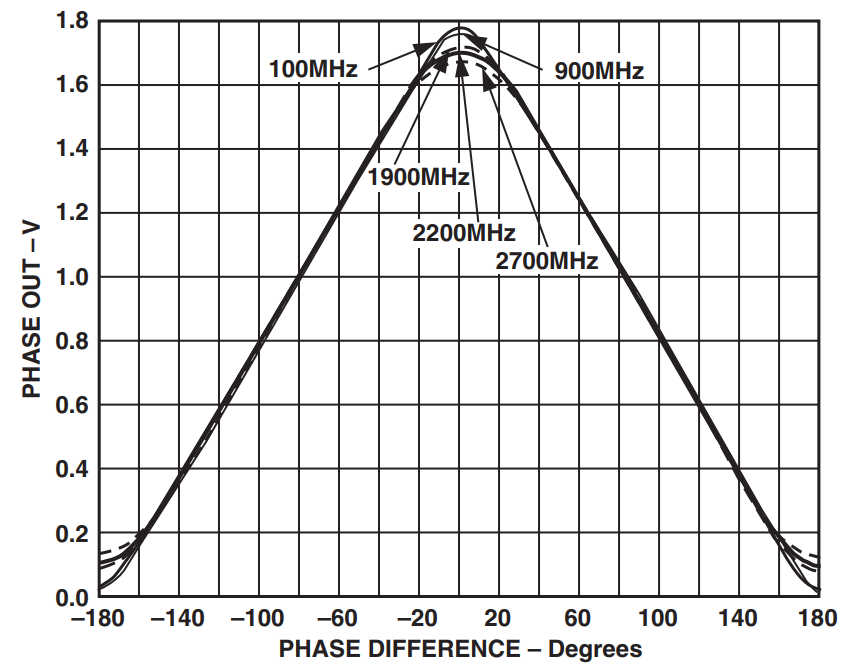
\includegraphics[width=0.6\linewidth]{ad8302_phase_frequency.png}
	\caption{VPHS Output over Frequency and Phase}
	\label{fig:ad8302_VPHS_frequency}
\end{figure}

\textbf{VPHS Log Conformance Error}\\
Like VMAG, VPHS has log conformance errors at the limits of the internal detectors, which manifest in increased errors when the phase difference is small between the two signals. This is highlighted in Figure \ref{fig:ad8302_VPHS_conformance}, which shows the phase error at 900 MHz can be up to 8 degrees when comparing the actual voltage output to the ideal linear fit. Measuring this flattening out of the output voltage and ensuring that the resolution of the sampling ADC is sufficiently high that it can detect the difference at low phase difference values is crucial, as this would allow reconstruction of the actual phase output with sufficient signal processing, which will be outlined in \S \ref{sec:implementation}. 
\begin{figure}[H]
	\centering
	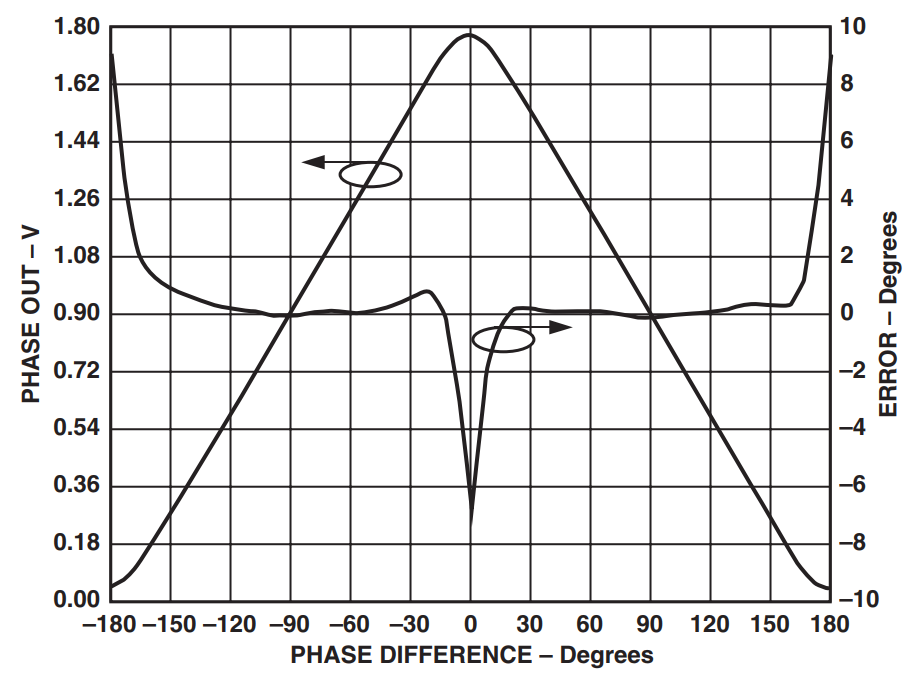
\includegraphics[width=0.6\linewidth]{ad8302_phase_error.png}
	\caption{VPHS Log Conformance Error at 900 MHz}
	\label{fig:ad8302_VPHS_conformance}
\end{figure}

\textbf{VPHS Frequency Dependence} \\
It should also be noted that as shown in Figure \ref{fig:ad8302_VPHS_frequency}, the log conformance error increases as a function of frequency. This will need to be compensated for in addition to the error increasing at small phase differences, and this will be covered in \S \ref{sec:implementation}. 

\subsubsection{Processor}
Sampling of the ADC, control of all onboard devices, along with communications with the host machine will require an embedded processor. As such, a microcontroller with sufficient pins and peripherals to connect to all required hardware, along with inbuilt USB and DSP instructions would be ideally suited to the task. Furthermore, an integrated ADC with at least 12 bits would be ideal, as this would ensure that sampling of the AD8302 could be done with the accuracy required. The STM32F373 series from STMicroelectronics is a great fit for this, as the line-up has 16 bit sigma-delta ADCs with programmable gain, a Cortex-M4 core which has DSP instructions capable of floating point add, multiply, and subtraction in a single clock, along with 64 to 256 Kbytes of flash, and packages with between 48 and 100 pins which will allow the hardware to scale once final specifications and code size are determined. 

\subsubsection{Power}
With components selected, it was determined that 100mA would be required at 5V, with approximately 300mA at 3V3 to power the devices. Due to the supply being 5V from USB, and the desire for low noise power rails due to the sensitive RF and analog measurements occurring, linear regulators were chosen to regulate the power down to 3V3 due to the low difference in input and output voltages and the desire for low output ripple. In particular, the LP5912 from Texas Instruments was chosen due to it's low output noise of 12$\mu$V\textsubscript{RMS} and high PSRR of 75dB at 1kHz, whilst costing less than \$2 in singles. Furthermore, the 3V3 rail was divided into analog and digital domains, with separate regulators for each and ferrite beads being used throughout to further reduce the influence of power supply noise on the system. 

\subsection{Firmware and Software}
\label{subsec:firmware_software}
Originally it was planned that the VNA would be a self contained device, capable of all correction and calibration required on device, and would expose itself via a serial port over which it could be controlled and calibrated data returned. However due to the complexity of this architecture and the time constraints on the project, most of the correction and calibration was moved over to the host computer, where Python tools such as NumPy, SciPy, and scikit-rf could be utilised to decrease the development time required, along with allowing decreased compute power for the embedded processor which would help reduce cost. 

Figure \ref{fig:sw_flowchart} shows the primary functions implemented in Software / Firmware, with the blue functions implemented host side in Python, and the purple functions running on the microprocessor in C. The interface between the two sides is done in plain text, and as such the VNA is capable of being controlled over a serial port if desired, with it returning a non calibrated, non phase corrected frequency / magnitude / phase triplet, which could be copied from the terminal and processed as desired. Further detail of the primary functional blocks will be discussed in \S \ref{sec:implementation}, as the architecture was developed during board bring-up and implementation. 

\begin{landscape}
	\begin{figure}[H]
		\centering
		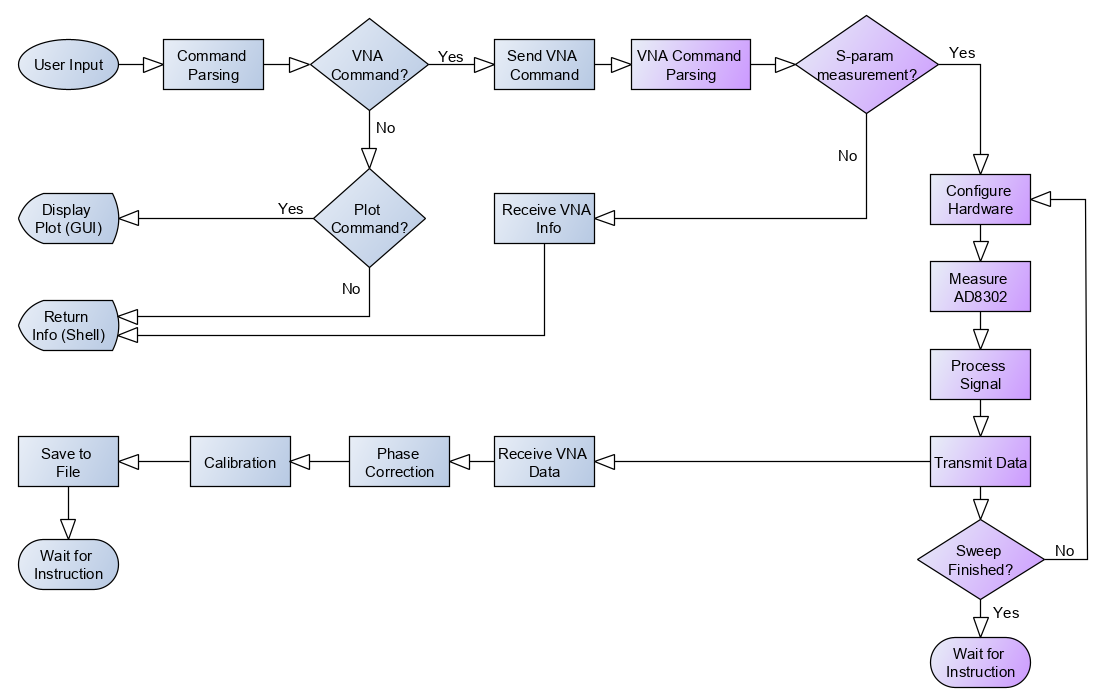
\includegraphics[width=\linewidth]{sw_flowchart.png}
		\caption{Flowchart of Primary Software / Firmware Steps}
		\label{fig:sw_flowchart}
	\end{figure}
\end{landscape}
	\pagebreak
	
 	\section{Implementation and Assembly}
 	\label{sec:implementation}
	With the high level design and primary component selection complete, detailed design of the VNA could begin. KiCad was used for all steps of the PCB design process, as it is a powerful free and open source EDA tool which is extensively used in the open source hardware community. For firmware, System Workbench for STM32 was utilised, as it provides open source tools such as GCC for Cortex-M cross compiling, OpenOCD for programming and debugging, precompiled and integrated in an Eclipse IDE, which makes getting firmware development started with a completely open source flow easy.

\subsection{Schematic Capture}
The first step in PCB design is schematic capture, where abstract representations of the components are joined together in a way which makes it easy to read and determine the desired functionality of the device. Due to development boards being designed earlier in the process, certain components such at the MAX2871 PLL, filter bank, and gain control circuitry were easily ported over into the new schematic, however due to issues such as a new amplifier needing to be designed in, along with the programmable attenuator being out of stock, changes were required to ensure that all components were able to be sourced in time, along with preforming as desired.

Other components such as the STM32 microcontroller, dual directional couplers, numerous status LEDs, and an auxiliary USB connection for powering DUTs and ECal units were also added to ensure that all required hardware was on device. Additionally numerous design for test additions such as 0 ohm resistors and DNP components, test points on all key signals, additional components in the PLL loop filter to allow an alternative PLL to be utilised, user addressable LEDs, unused pints being broken out, power rail LEDs, numerous ground points along with a unused UART connection were all designed in to make bring-up of the board as easy as possible. The completed schematic can be found in Appendix \ref{appen:vna_design_files}, Figures \ref{fig:vna_schematic_overview} through \ref{fig:vna_schematic_power}.

\subsection{Layout Planning}
Before the PCB layout can begin, there are a few key steps and decisions which need to made which will place constraints on the design of the PCB. Firstly, component footprints were associated with the relevant schematic symbols, with footprints being designed where KiCad did not have them in the standard library. Furthermore 3D models for every component were either loaded from KiCad, sourced from the distributor, or drawn from mechanical drawings, as this would allow for mechanical fit with an enclosure to be confirmed later in the design process. 

With all the components imported into CAD, the approximate size of the PCB was able to be determined. This allowed for COTS aluminium case options to be explored, and once an enclosure was found which was large enough for the PCB to fit, the exact dimensions of the PCB were able to be fixed to that dimension, allowing the positioning of connectors, mounting holes, and other key features of the PCB to be placed. 

The PCB stackup and manufacturer also needed to be determined, as this plays a key role in the cost of the boards, along with key PCB features such as minimum space / trace, via size, and the with of a 50 ohm microstrip trace. Due to cost and prior experience, JLCPCB was chosen as the manufacturer, and their 4 layer FR4 "JLC7628" stackup (Table \ref{table:pcb_stackup}) was chosen as it is a very common stackup well suited to the feature and component sizes used by the components, along with the ability for it to be ordered from other manufacturers with ease. Furthermore, a Signal / GND / PWR / Signal configuration would be designed for during layout, with flood fills of ground on layers 1 and 4. 

\begin{table}[h!]
	\centering
	\caption{Chosen PCB stackup}
	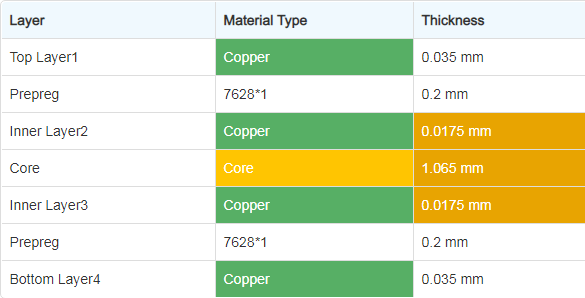
\includegraphics[width=0.8\linewidth]{jlc_stackup.png}
	\label{table:pcb_stackup}
\end{table}

Other key feature sizes for the chosen stackup and manufacturing process are outlined in Table \ref{table:pcb_specs}. It should be noted that whilst JLCPCB are able to do quite small trace / space and via drill size, 6 / 6 trace / space and 0.25 / 0.5 drill / via were chosen for the design, as this would allow it to be fabricated at common fabricators such as OSHPark and PCBWay without paying for advanced processes. 
\begin{table}[h!]
	\caption{Key specifications of PCB design rules and feature size}
	\label{table:pcb_specs}
	\centering
	\begin{tabular}{|c|c|}
		\hline
		\textbf{Feature}                          & \textbf{Dimension} \\ \hline
		Min Trace / Space                         & 0.15 mm (6 mil)   \\ \hline
		Min Via Drill Size                        & 0.25 mm (10 mil)     \\ \hline
		Min Via Diameter                          & 0.5 mm (20 mil)   \\ \hline
		50 $\Omega$ Microstrip Width              & 0.29 mm (11.5 mil) \\ \hline
		Blind / Buried / Micro Via                & Not Available \\ \hline
	\end{tabular}
\end{table} 

\subsection{PCB Layout}
Given the mechanical dimensions, stackup, and design rules have be determined, these parameters can be loaded into KiCad and the PCB can be laid out. An image of the laid out board can be found in Figure \ref{fig:pcb_layout}, with a 3D render available in Figure \ref{fig:pcb_render}.

Given the operating frequencies seen on the board, a number of key layout considerations were taken into account to ensure optimal function of the board, and are detailed below.
\begin{itemize}
	\item \textbf{50 $\Omega$ RF Traces} need to be kept along the signal path to ensure a good match between components, and this is achieved on this board through using a 0.29 mm microstrip on layer 1 over a continuous ground pour on layer 2. 
	\begin{itemize}
		\item Furthermore, compensation for extra capacitance introduced under the large pads of the directional couplers and SMA connectors need to occur, as otherwise there will be added capacitance which will decrease the match of the transmission line. This can be seen in Figure \ref{fig:pcb_cap_comp}, where the ground fill has been removed to significantly reduce the inter-planar capacitance between layers 1 and 2, to ensure a consistent characteristic impedance. 
		\item When a layer change is required for the RF signal, care must be taken to ensure there is a low impedance path between reference layers. This can be seen on the first directional coupler as shown in Figure \ref{fig:pcb_layer_change}, where the RF travels from the bottom left on layer 1, through a via to layer 4, and back to layer 1 in the top right hand corner. Stitching vias can be seen close to the signal via to ensure a low inductance path between the two reference planes, along with the signal vias being optimised to have a 50 $\Omega$ impedance to reduce impedance discontinuity. 
		
		Unfortunately a mistake was made during layout in that the signal was routed on layer 4 instead of 3, as with the signal on 4 it's reference plane is layer 3, VCC, which does not have a low inductance path to layer 2, as the closets decoupling caps are located in the top left of the image, near the 8 pin DFN IC. Ideally the signal would have been routed on layer 3,  allowing the ground pour on layer 4 to be the reference plane, with the multiple vias providing a low inductance path between the two planes. Fortunately, due to upper bounds of the frequencies seen on the board at 1.25 GHz, this is not a major issue which has caused issues with the function of the device. 
		\item Low impedance between layers was also ensured through the use of ample stitching vias, both around the signal path and the entire board. 
	\end{itemize}
	\item \textbf{EMI Reduction} is crucial to ensure that there is no coupling of unwanted signals onto the key signals. This has been achieved by routing the digital signals on the left side of the board, allowing the RF and analog signals from the AD8302 to have as much clearance as possible from the digital signals. Furthermore, the output drivers on the STM32 were set to a low slew rate, as this will decrease the frequency content seen when a signal is switched. 
	\item \textbf{Power Integrity} was achieved through the use of linear regulators to decrease noise on the power rails, low inductance connections to components through large power planes and multiple vias when changing layers to ensure the added inductance is kept to a minimum. Furthermore, ensuring the decoupling capacitors specified in application notes for each component are placed close the power pins, with the smaller capacitors closer to the pin, and a dedicated via for each capacitor placed as close as possible to the pad ensures that the impedance and noise seen at the power pin to each component is kept at a minimum, which leads to optimum performance of the IC and minimal coupling of noise onto the RF and analog signals.
	\item \textbf{Following reference layouts} ensured that the device would preform as specified on the data sheet, along with being able to rule out bad component placement and routing as possible causes for improper function of device. Where reference designs were not available, best RF layout practices including those described above were utilised to ensure optimal performance of the device.  
\end{itemize} 

\begin{figure}[H]
	\centering
	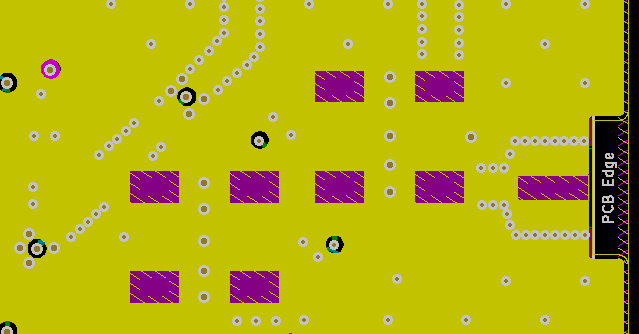
\includegraphics[width=0.45\linewidth]{ground_cutouts.png}
	\caption{Ground cut-outs under large pads to reduce inter-planar capacitance and ensure a 50 $\Omega$ transmission line}
	\label{fig:pcb_cap_comp}
\end{figure}

\begin{figure}[H]
	\centering
	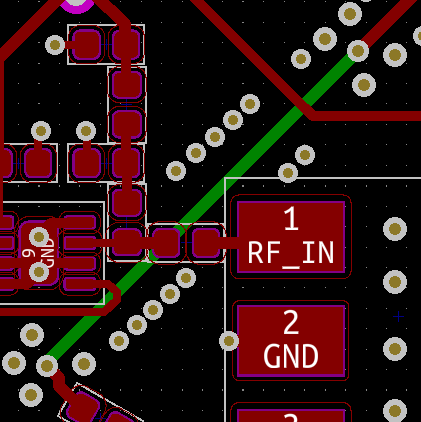
\includegraphics[width=0.3\linewidth]{layer_change.png}
	\caption{Layer change mistake on the signal path}
	\label{fig:pcb_layer_change}
\end{figure}

\begin{landscape}
	\begin{figure}
		\centering
		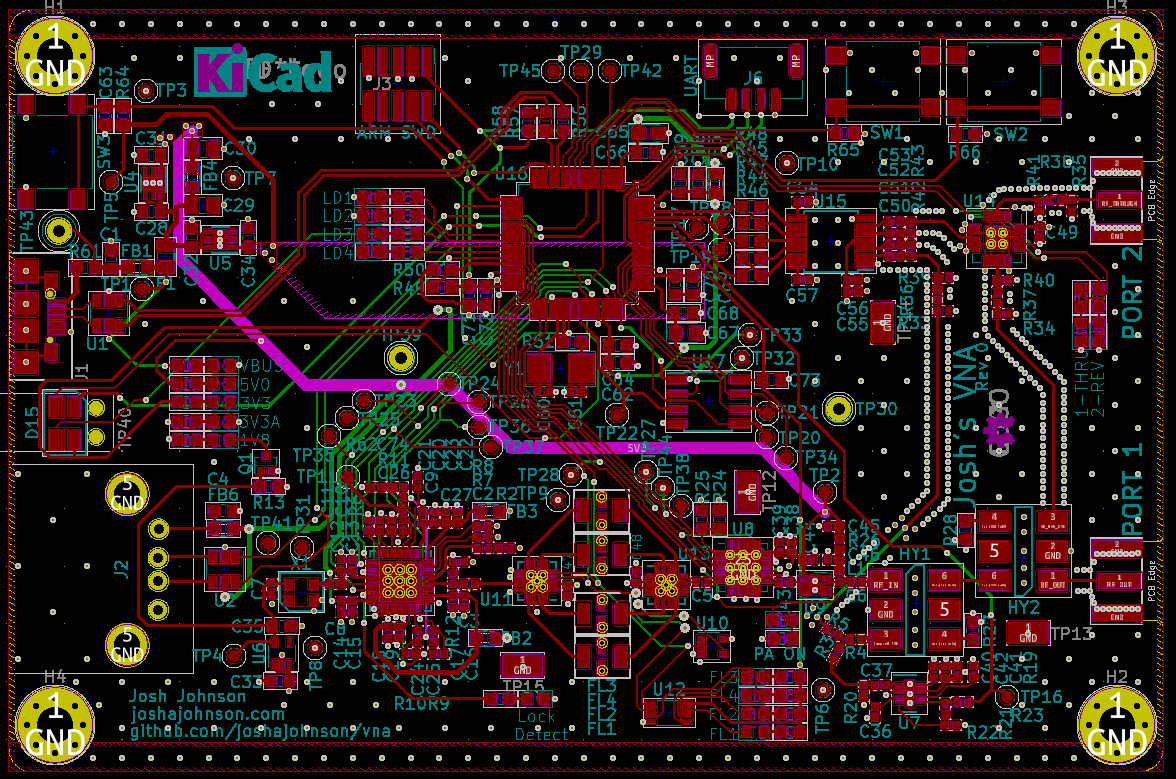
\includegraphics[width=\linewidth]{pcb_layout.png}
		\caption{PCB Layout, with Red = Layer 1, Yellow = Layer 2, Pink = Layer 3, Green = Layer 4. Flood fill of each layer is not shown.}
		\label{fig:pcb_layout}
	\end{figure}
\end{landscape}

\subsection{Mechanical Design}
To ensure there will be no mechanical clearance issues, a STEP was exported from KiCad in to Fusion360 and placed into a model of the extrusion, and is was seen that there were no mechanical issues. Having the 3D model in MCAD, together with the decision to use an extruded aluminium enclosure results in easy design of custom front and rear panels, as key features from the 3D model can be referenced when designing cut-outs for the connectors and light pipe. DXFs were exported from Fusion360 back into KiCad where they had silkscreen added, and they were then sent off to be manufactured with the main VNA PCB. Renders of the front and rear panels can be found in Figures \ref{fig:pcb_front_render} and \ref{fig:pcb_rear_render}, and the assembled VNA without the top extruded section in Figure \ref{fig:pcb_assembled}.

\begin{figure}[H]
	\centering
	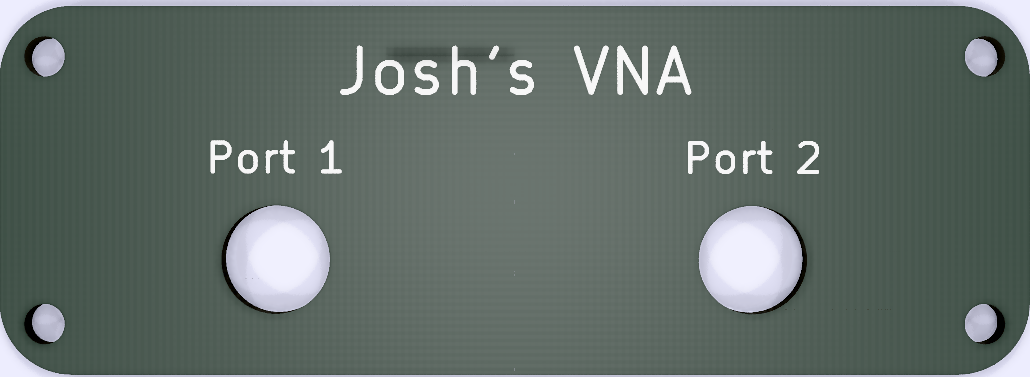
\includegraphics[width=0.8\linewidth]{frontPanel.png}
	\caption{Render of the VNA Front Panel}
	\label{fig:pcb_front_render}
\end{figure}

\begin{figure}[H]
	\centering
	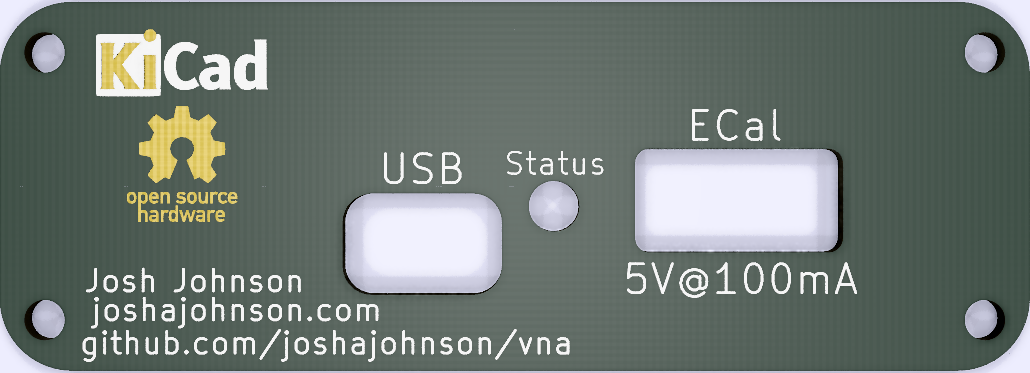
\includegraphics[width=0.8\linewidth]{rearPanel.png}
	\caption{Render of the VNA Rear Panel}
	\label{fig:pcb_rear_render}
\end{figure}

\begin{figure}[H]
	\centering
	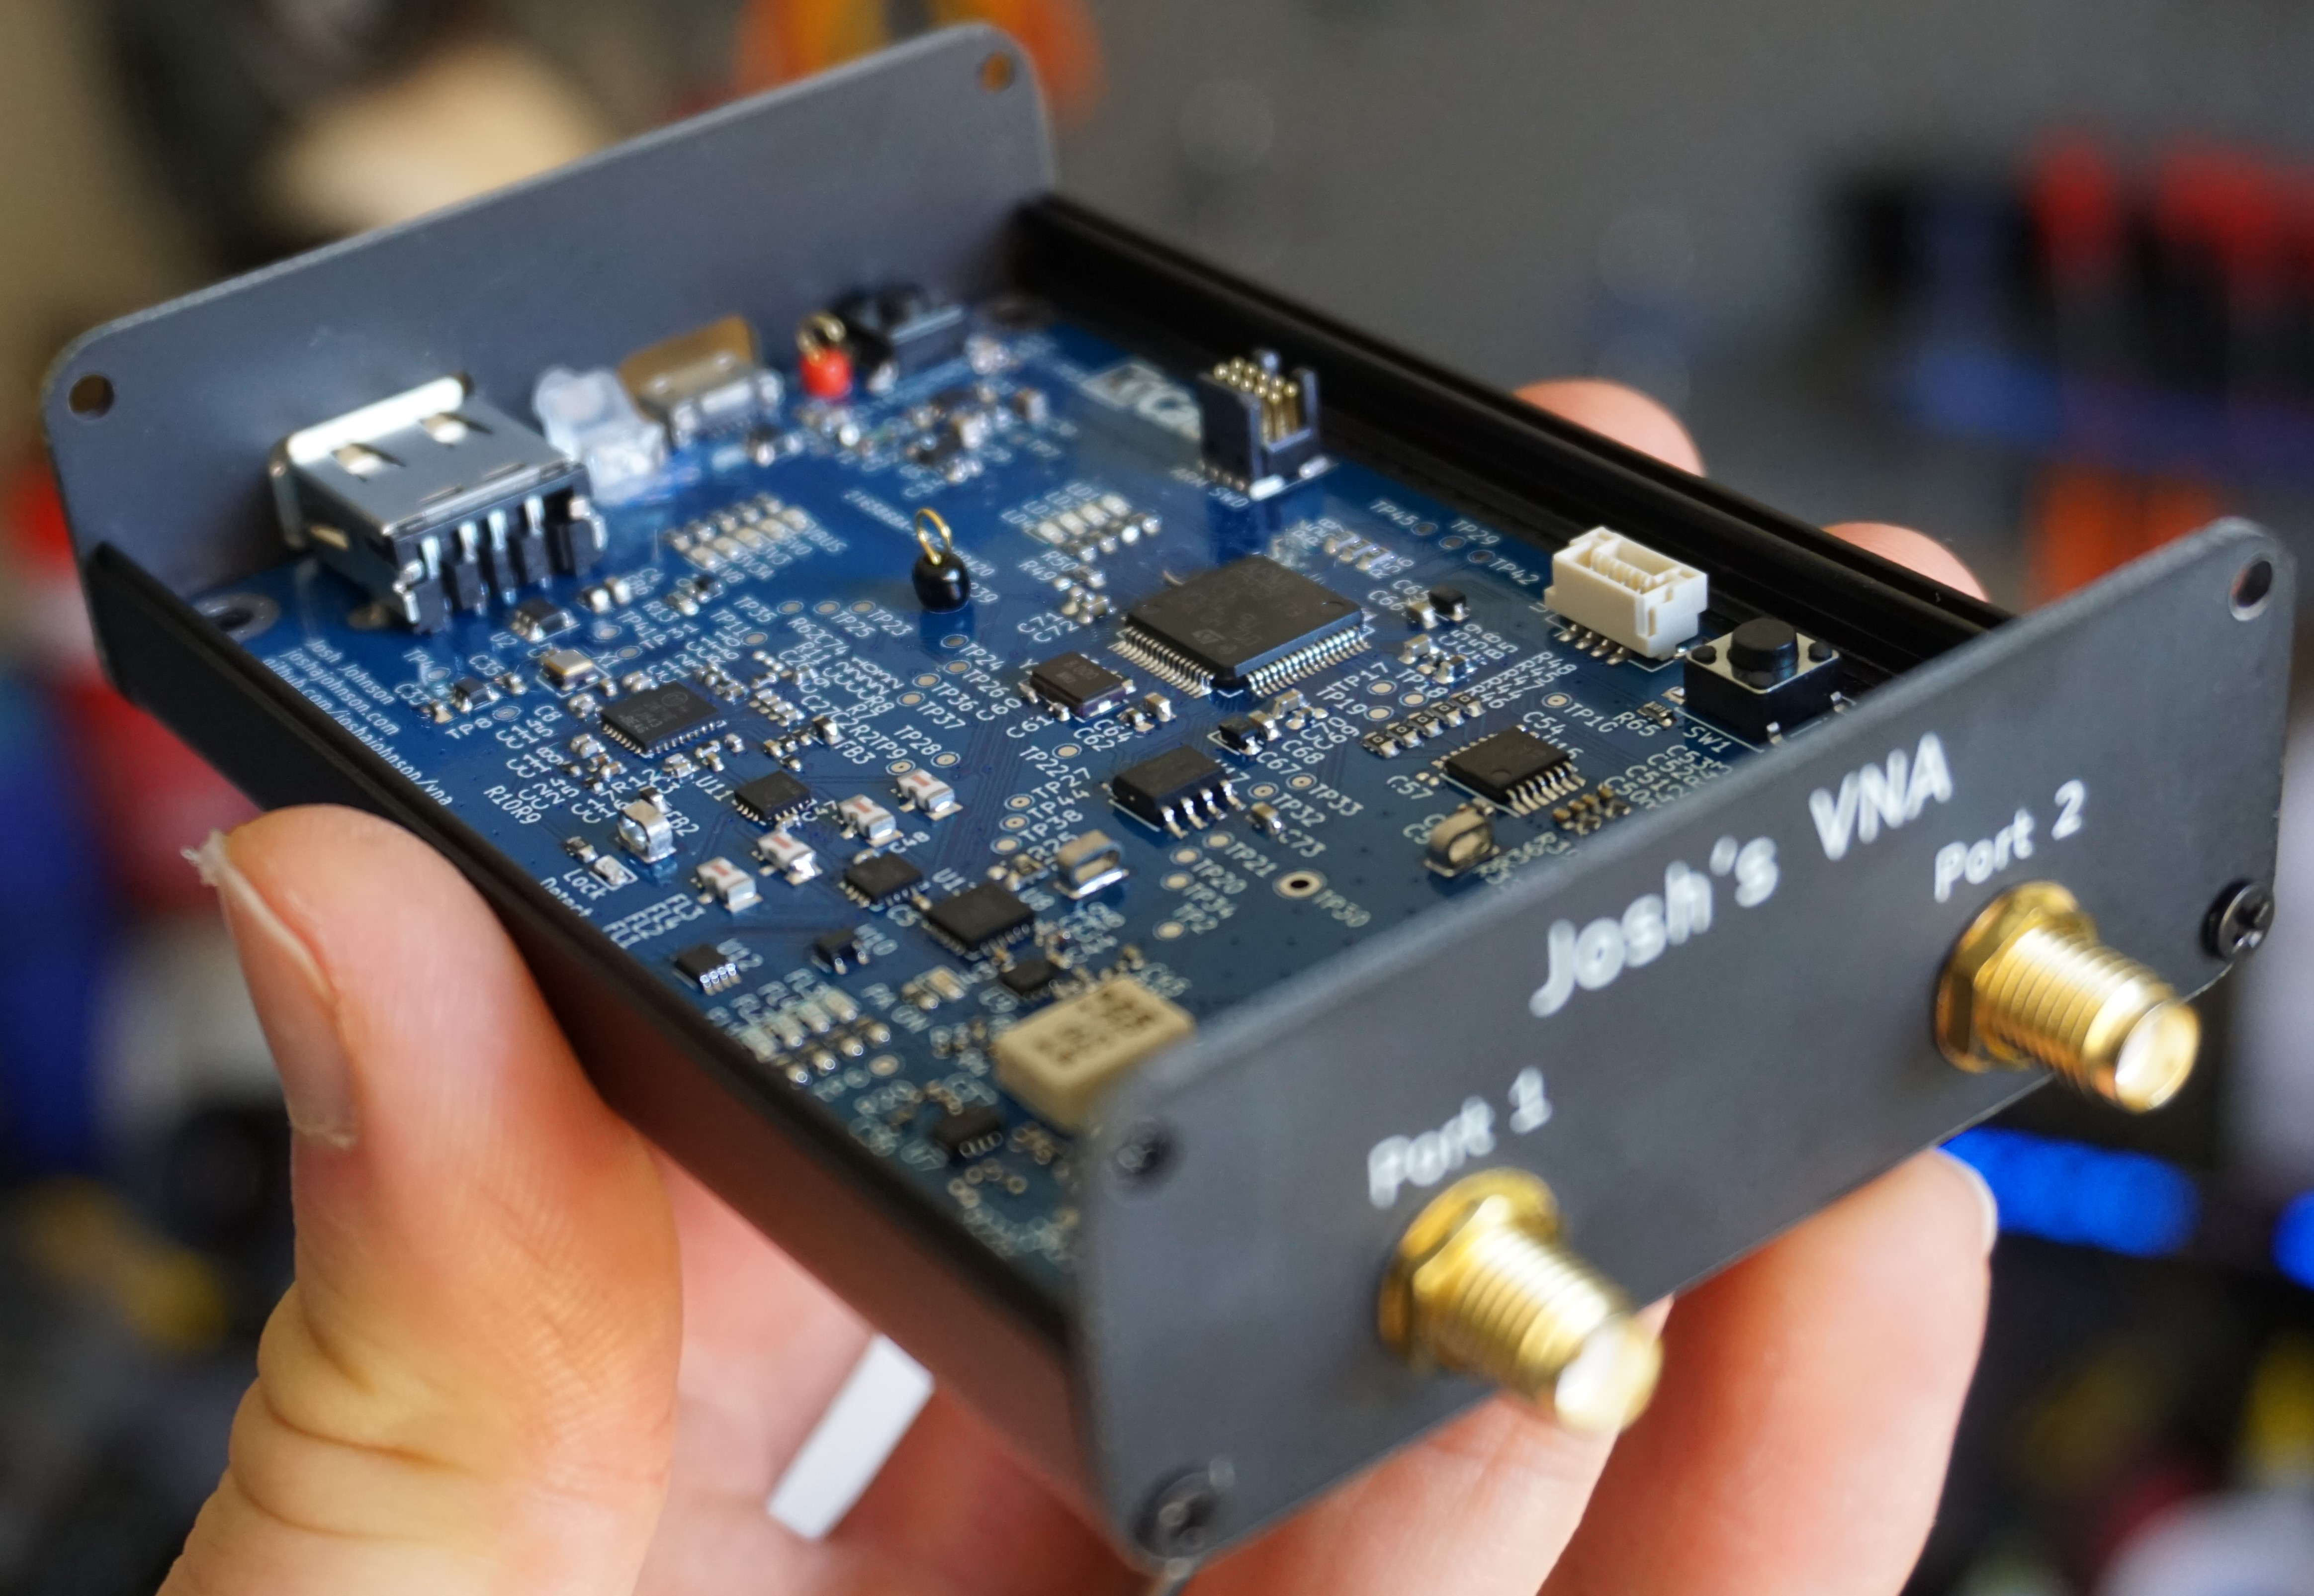
\includegraphics[width=\linewidth]{assembledVNA.jpg}
	\caption{Assembled VNA in enclosure, with top section removed}
	\label{fig:pcb_assembled}
\end{figure}

\subsection{Assembly + Bill of Materials}
Upon arrival of assembled PCBs and solder paste stencil, assembly was undertaken. This followed a fairly standard SMT process, with solder paste being deposited onto the PCB through the use of a stencil, placement of components under a microscope due to their size (down to 0402 and 0.5 mm QFN), and reflow in a reflow oven. Rework was required for a few components due to tomb stoning, along with some shorted pins on the QFNs, and hand soldering of the through hole components and SMA connectors. The board was then cleaned in an ultrasonic cleaner to remove any remaining flux, and left to dry for an hour in the reflow oven. This process went quite smoothly with the whole process taking less than 6 hours from start to finish. 

Table \ref{table:BOM} outlines the cost to manufacture one VNA, with removal of components such as debug headers and ground test points which are only required on the development boards. It should be noted that the per board cost at quantity 10 is reduced to \$204.78 due to the cost of PCBs being split between multiple boards and a slight reduction in component price, and that if free samples are requested from Analog Devices and Maxim and no case is utilised, the cost of assembling a VNA can be as little as \$185.37. Pricing is correct as of 10/10/19.


\begin{table}[H]
	\caption{Bill of Materials for VNA}
	\label{table:BOM}
	\centering
	\begin{tabular}{|c|c|c|c|c|}
		\hline
		\textbf{Quantity} & \textbf{Part Number}       & \textbf{Description}     & \textbf{\begin{tabular}[c]{@{}c@{}}Price Each \\ (\$AUD)\end{tabular}} & \textbf{\begin{tabular}[c]{@{}c@{}}Per Board \\ (\$AUD)\end{tabular}} \\ \hline
		1                 & MAX2871                    & PLL with VCO             & 18.95                                                                 & 18.95                                                                     \\ \hline
		1                 & ASTXR-12         & Reference Clock          & 4.75                                                                  & 4.75                                                                      \\ \hline
		2                 & PE42440                    & SP4T Switch              & 1.93                                                                  & 3.87                                                                      \\ \hline
		1                 & LFCN-105+                  & Low Pass Filter          & 15.27                                                                 & 15.27                                                                     \\ \hline
		1                 & LFCN-225+                  & Low Pass Filter          & 11.45                                                                 & 11.45                                                                     \\ \hline
		1                 & LFCN-400+                  & Low Pass Filter          & 11.45                                                                 & 11.45                                                                     \\ \hline
		1                 & LFCN-1000+                 & Low Pass Filter          & 7.61                                                                  & 7.61                                                                      \\ \hline
		1                 & TRF37A75                   & Power Amplifier          & 2.84                                                                  & 2.83                                                                      \\ \hline
		1                 & SKY12347-362LF             & Attenuator  & 10.04                                                                 & 10.04                                                                     \\ \hline
		2                 & ADC-15-4+                  & Directional Coupler      & 19.21                                                                 & 38.43                                                                     \\ \hline
		1                 & AD8319                     & Log Power Detector       & 8.69                                                                   & 8.69                                                                       \\ \hline
		1                 & AD8302                     & Gain Phase Detector      & 45.10                                                                   & 45.10                                                                       \\ \hline
		1                 & F2923                      & SPDT RF Switch           & 8.20                                                                  & 8.20                                                                      \\ \hline
		2                 & SMA                        & DUT Connector            & 2.12                                                                  & 4.24                                                                      \\ \hline
		1                 & Micro USB                  & Connection to PC         & 0.12                                                                  & 0.12                                                                      \\ \hline
		1                 & USB A                      & External Connection & 0.42                                                                  & 0.42                                                                     \\ \hline
		2                 & LP5912                     & 3V3 LDO                  & 2.01                                                                 & 4.02                                                                     \\ \hline
		1                 & MIC5366-1.8                & 1V8 LDO                  & 0.37                                                                  & 0.37                                                                      \\ \hline
		1                 & Polyfuse                   & Input protection   & 0.39                                                                  & 0.39                                                                      \\ \hline
		2                 & TPD2S017                   & ESD Protection           & 1.05                                                                  & 2.11                                                                      \\ \hline
		1                 & STM32F373              & Microcontroller           & 8.87                                                                 & 8.87                                                                      \\ \hline
		1                 & 8 MHz Crystal              & For MCU                  & 0.83                                                                  & 0.83                                                                      \\ \hline
		1                 & RGB LED                    & Status LED               & 0.88                                                                  & 0.88                                                                      \\ \hline
		1                 & Assorted Capacitors        &                          & 2.20                                                                    & 2.20                                                                        \\ \hline
		1                 & Assorted Passives &                          & 1.10                                                                    & 1.10                                                                        \\ \hline
		1                 & VNA PCB                    & (Price for 5)            & 45.67                                                                 & 45.67                                                                     \\ \hline
		1                 & Enclosure                  &                          & 8.28                                                                  & 8.22                                                                      \\ \hline
		2                 & Front/Rear Panels         & (Price for 5)            & 3.26                                                                  & 6.53                                                                      \\ \hline
		1                 & Light Pipe                 &                          & 0.98                                                                   & 0.98                                                                       \\ \hline
		&                            &                          &                                                                        &                                                                            \\ \hline
		&                            &                          & Total Cost                                                             & 272.88                                                                    \\ \hline
	\end{tabular}
\end{table} 

\subsection{Board Errata}
There were a few issues found during board bring-up which required hardware changes. Firstly, buttons which were placed on device to aide debugging were drawn up incorrectly in the schematic and resulted in both sides of the button being tied to ground. This was resolved by lifting pads of the button and connecting them to 3V3 as required.

A more challenging issue to resolve was found in that upon reset of the microcontroller, it would not re-enumerate with the host however Windows would still show it as connected. Following some googling it was found that Windows requires the 1K5 pull-up resistor on D+ to be pulled to ground during reset, as this triggers re-enumeration of the device. This issue was resolved by connecting the pull-up resistor to an unused GPIO pin which upon start-up would pull the pin low, wait a few milliseconds, and then assert it high to force re-enumeration. 

The only other hardware issue found on the board was to do with the configuration of the MAX2871's output signals. Upon bring-up of the transmit chain, it was noted that the RF power was far too low and this was narrowed down to the output of the MAX2871 being tens of dB too low. The issue was found to be incorrect termination of the unused RF- output to ground through a 50$\Omega$ resistor, instead of being pulled up to 3V3 through a resistor before being tied to ground. This was resolved with reworking some 0402 components and adding a flying wire as shown in Figure \ref{fig:max_rework}.

\begin{figure}[H]
	\centering
	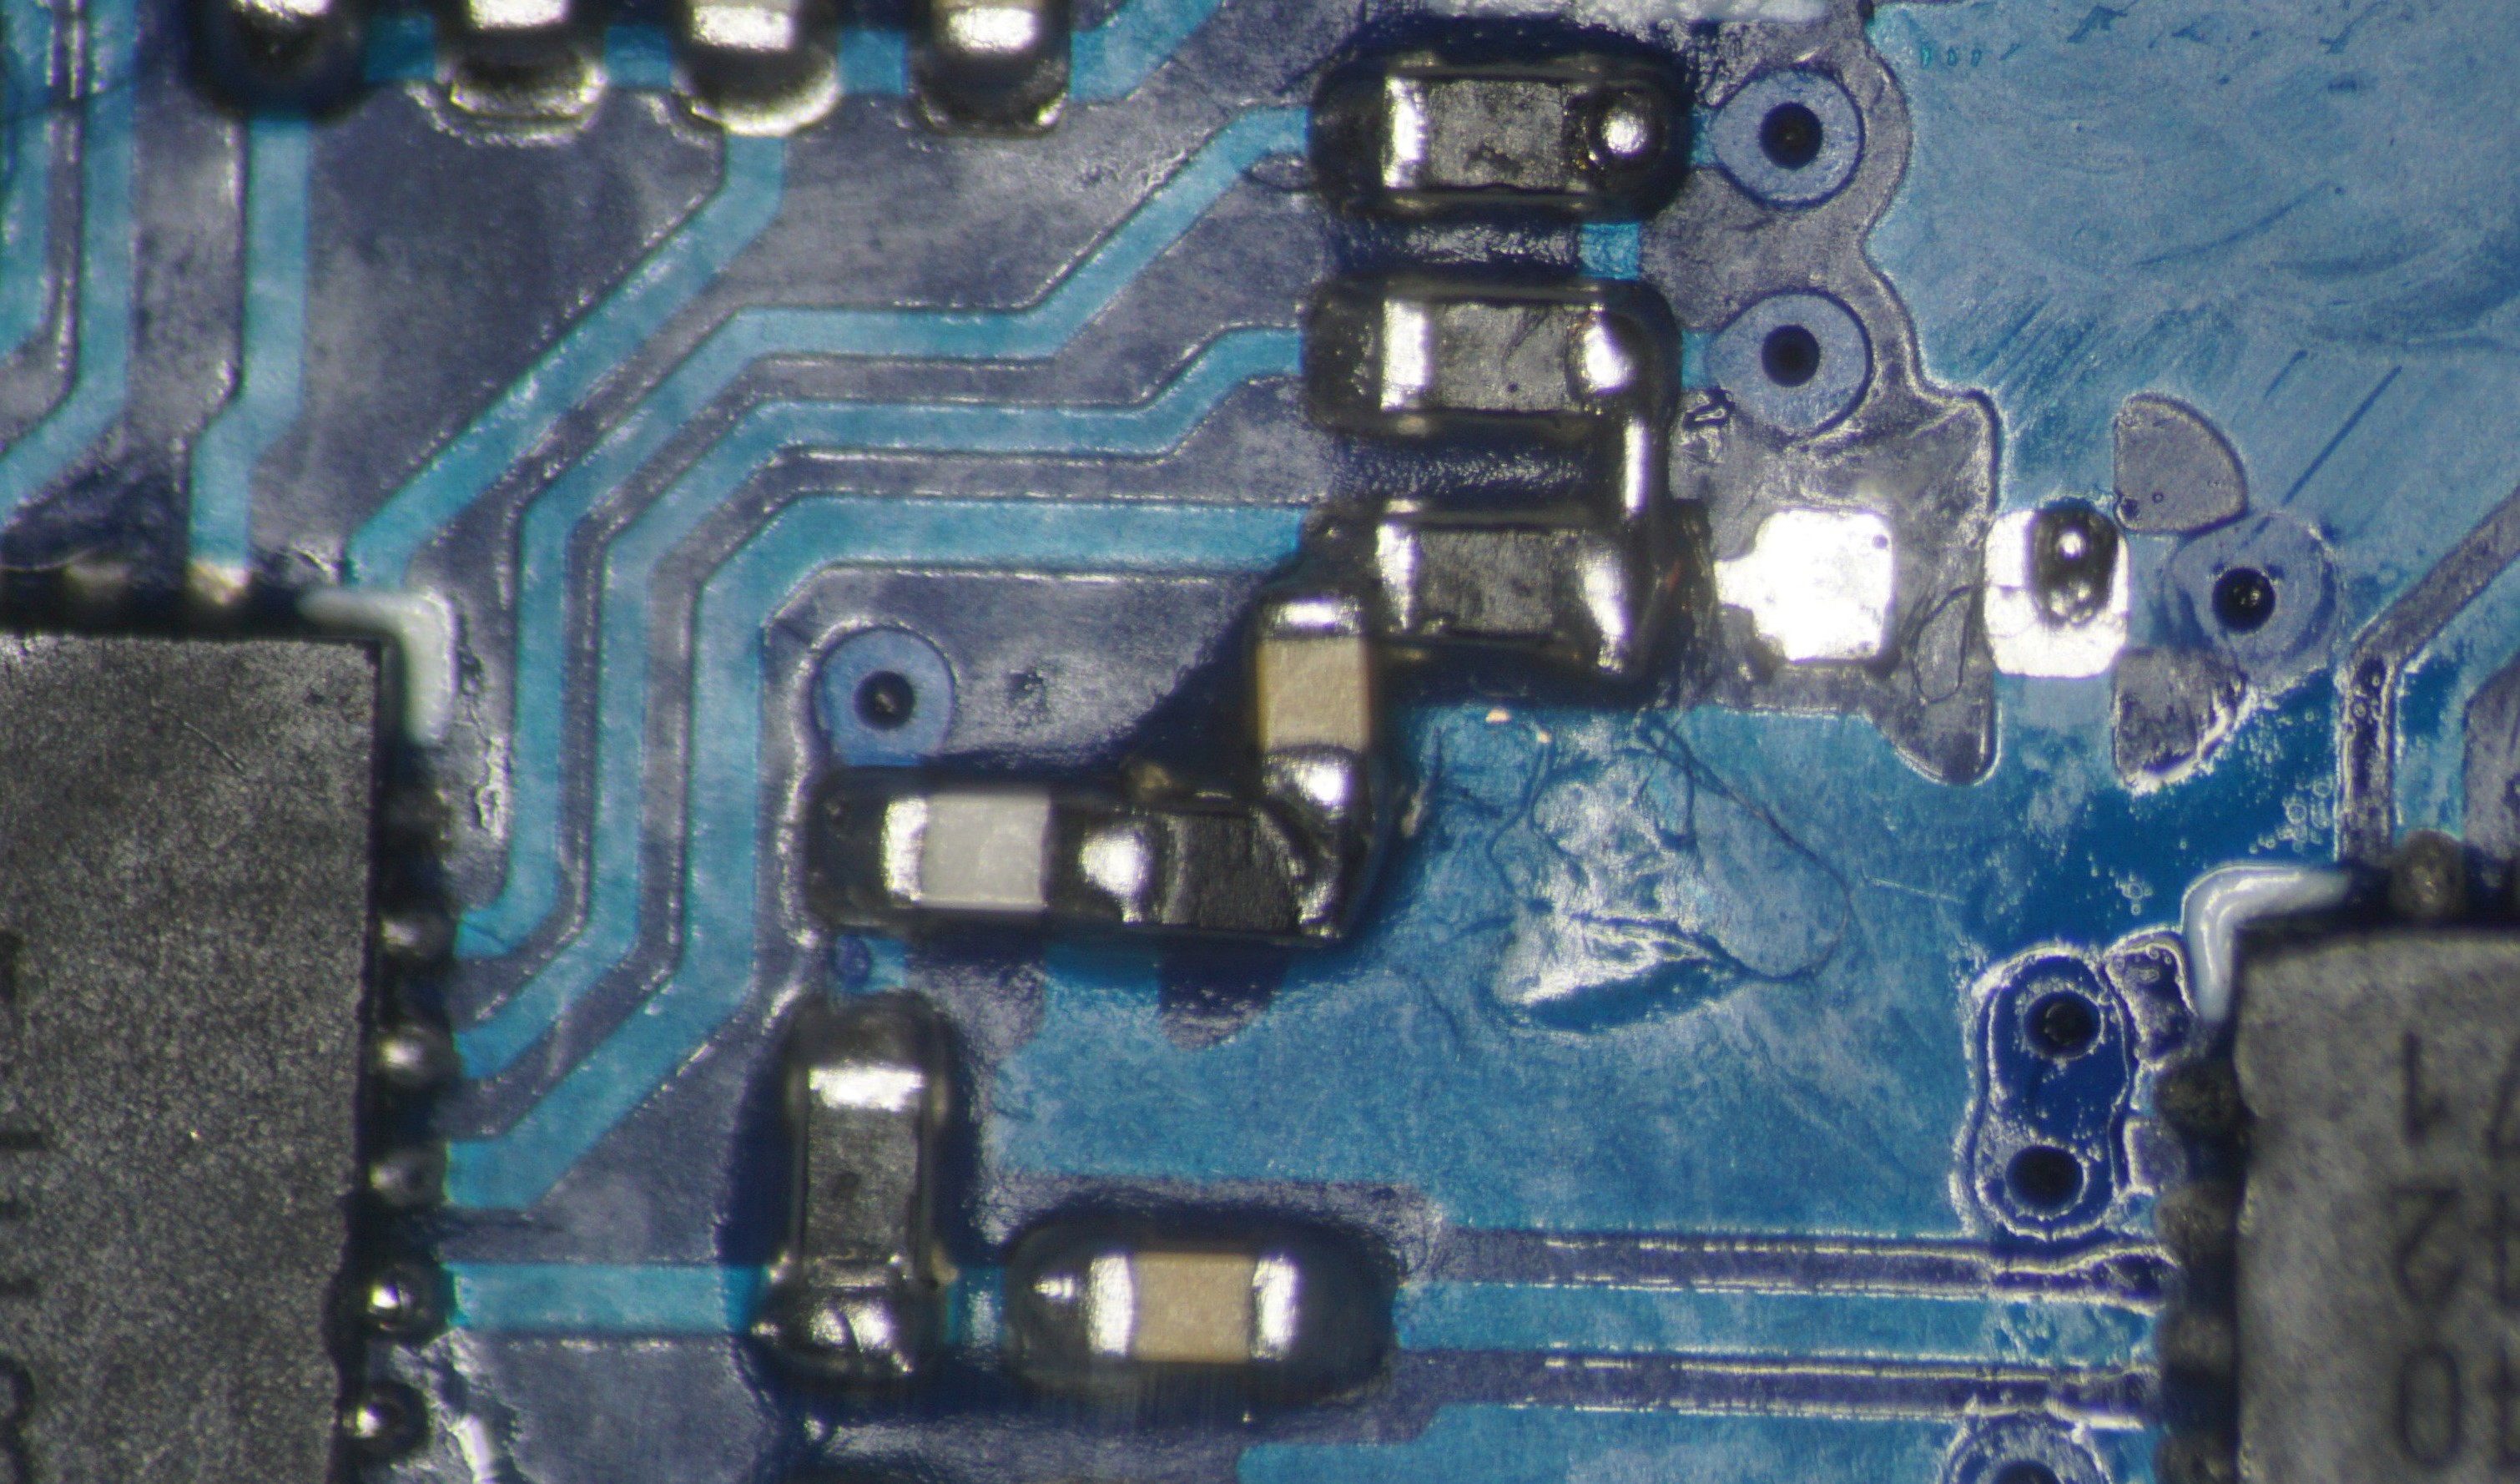
\includegraphics[width=0.65\linewidth]{max_rework.jpg}
	\caption{Rework of the MAX2871 RF- output}
	\label{fig:max_rework}
\end{figure}

\subsection{ECal Design}
To aide with use of the VNA, a low cost ECal unit was designed which switches in calibrations standards based on commands from the VNA. It is controlled through the use of a USB cable, where the data pins are either I2C so a port expander with up to 16 control pins can be utilised, or GPIO, so a SP4T switch can be controlled by toggling two pins. Furthermore, the design utilises a two layer board with a grounded coplanar waveguide for the RF trace, as the trace width required on a 1.6mm substrate for a 50$\Omega$ transmission line is far too wide for easy design and would result in increased impedance mismatch during tapering of the trace to meet the 0.3mm pads of the QFN switch. 

For the ECal to be utilised, it's S-parameters must be measured with a VNA as this effectively transfers the calibration from the VNA's calibration standards to the ECal unit, and from there the ECal's generated touchstone file can be used as a reference of the expected frequency response. Unfortunately due to the VNA accessed at ANU not having a SMA calibration kit it the ECal was not able to be used during development, but it has been shown to function and as such if it was measured there is nothing stopping it from being used as a substitute for discrete calibration standards.

The schematic for the RF section of the VNA can be found in Figure \ref{fig:ecal_schematic}, with an image of it in Figure \ref{fig:ecal_photo}.

\begin{figure}[H]
	\centering
	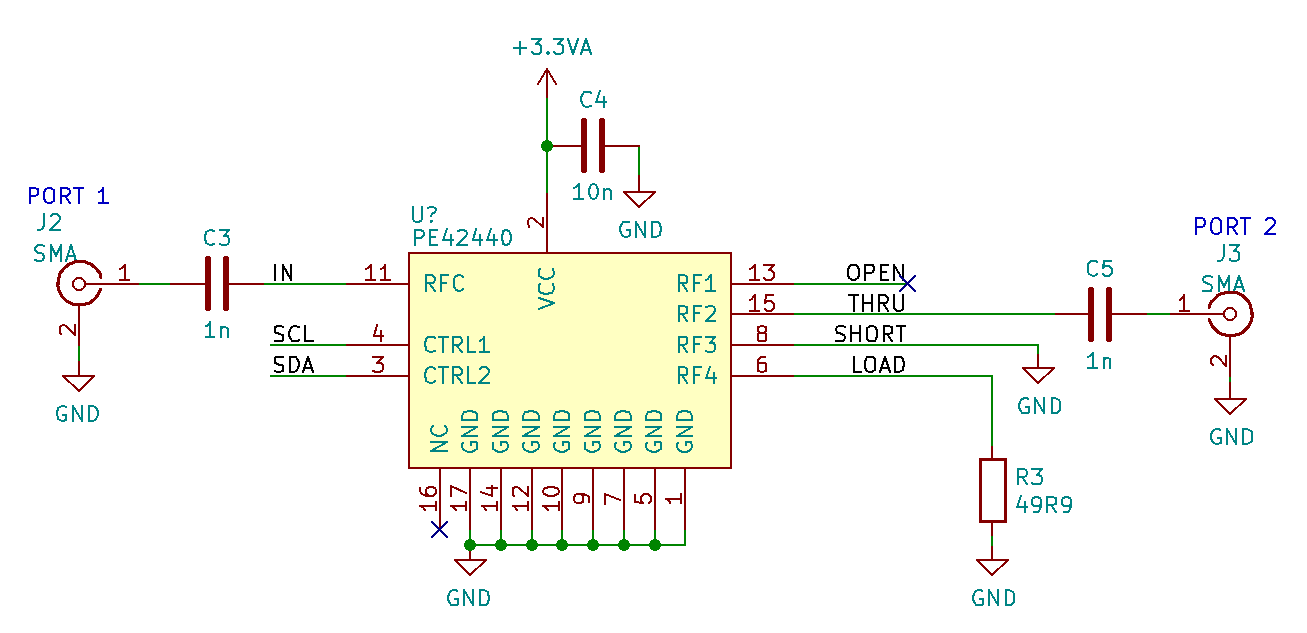
\includegraphics[width=0.9\linewidth]{ecal_schematic.png}
	\caption{Schematic of the ECal RF circuit}
	\label{fig:ecal_schematic}
\end{figure}

\begin{figure}[H]
	\centering
	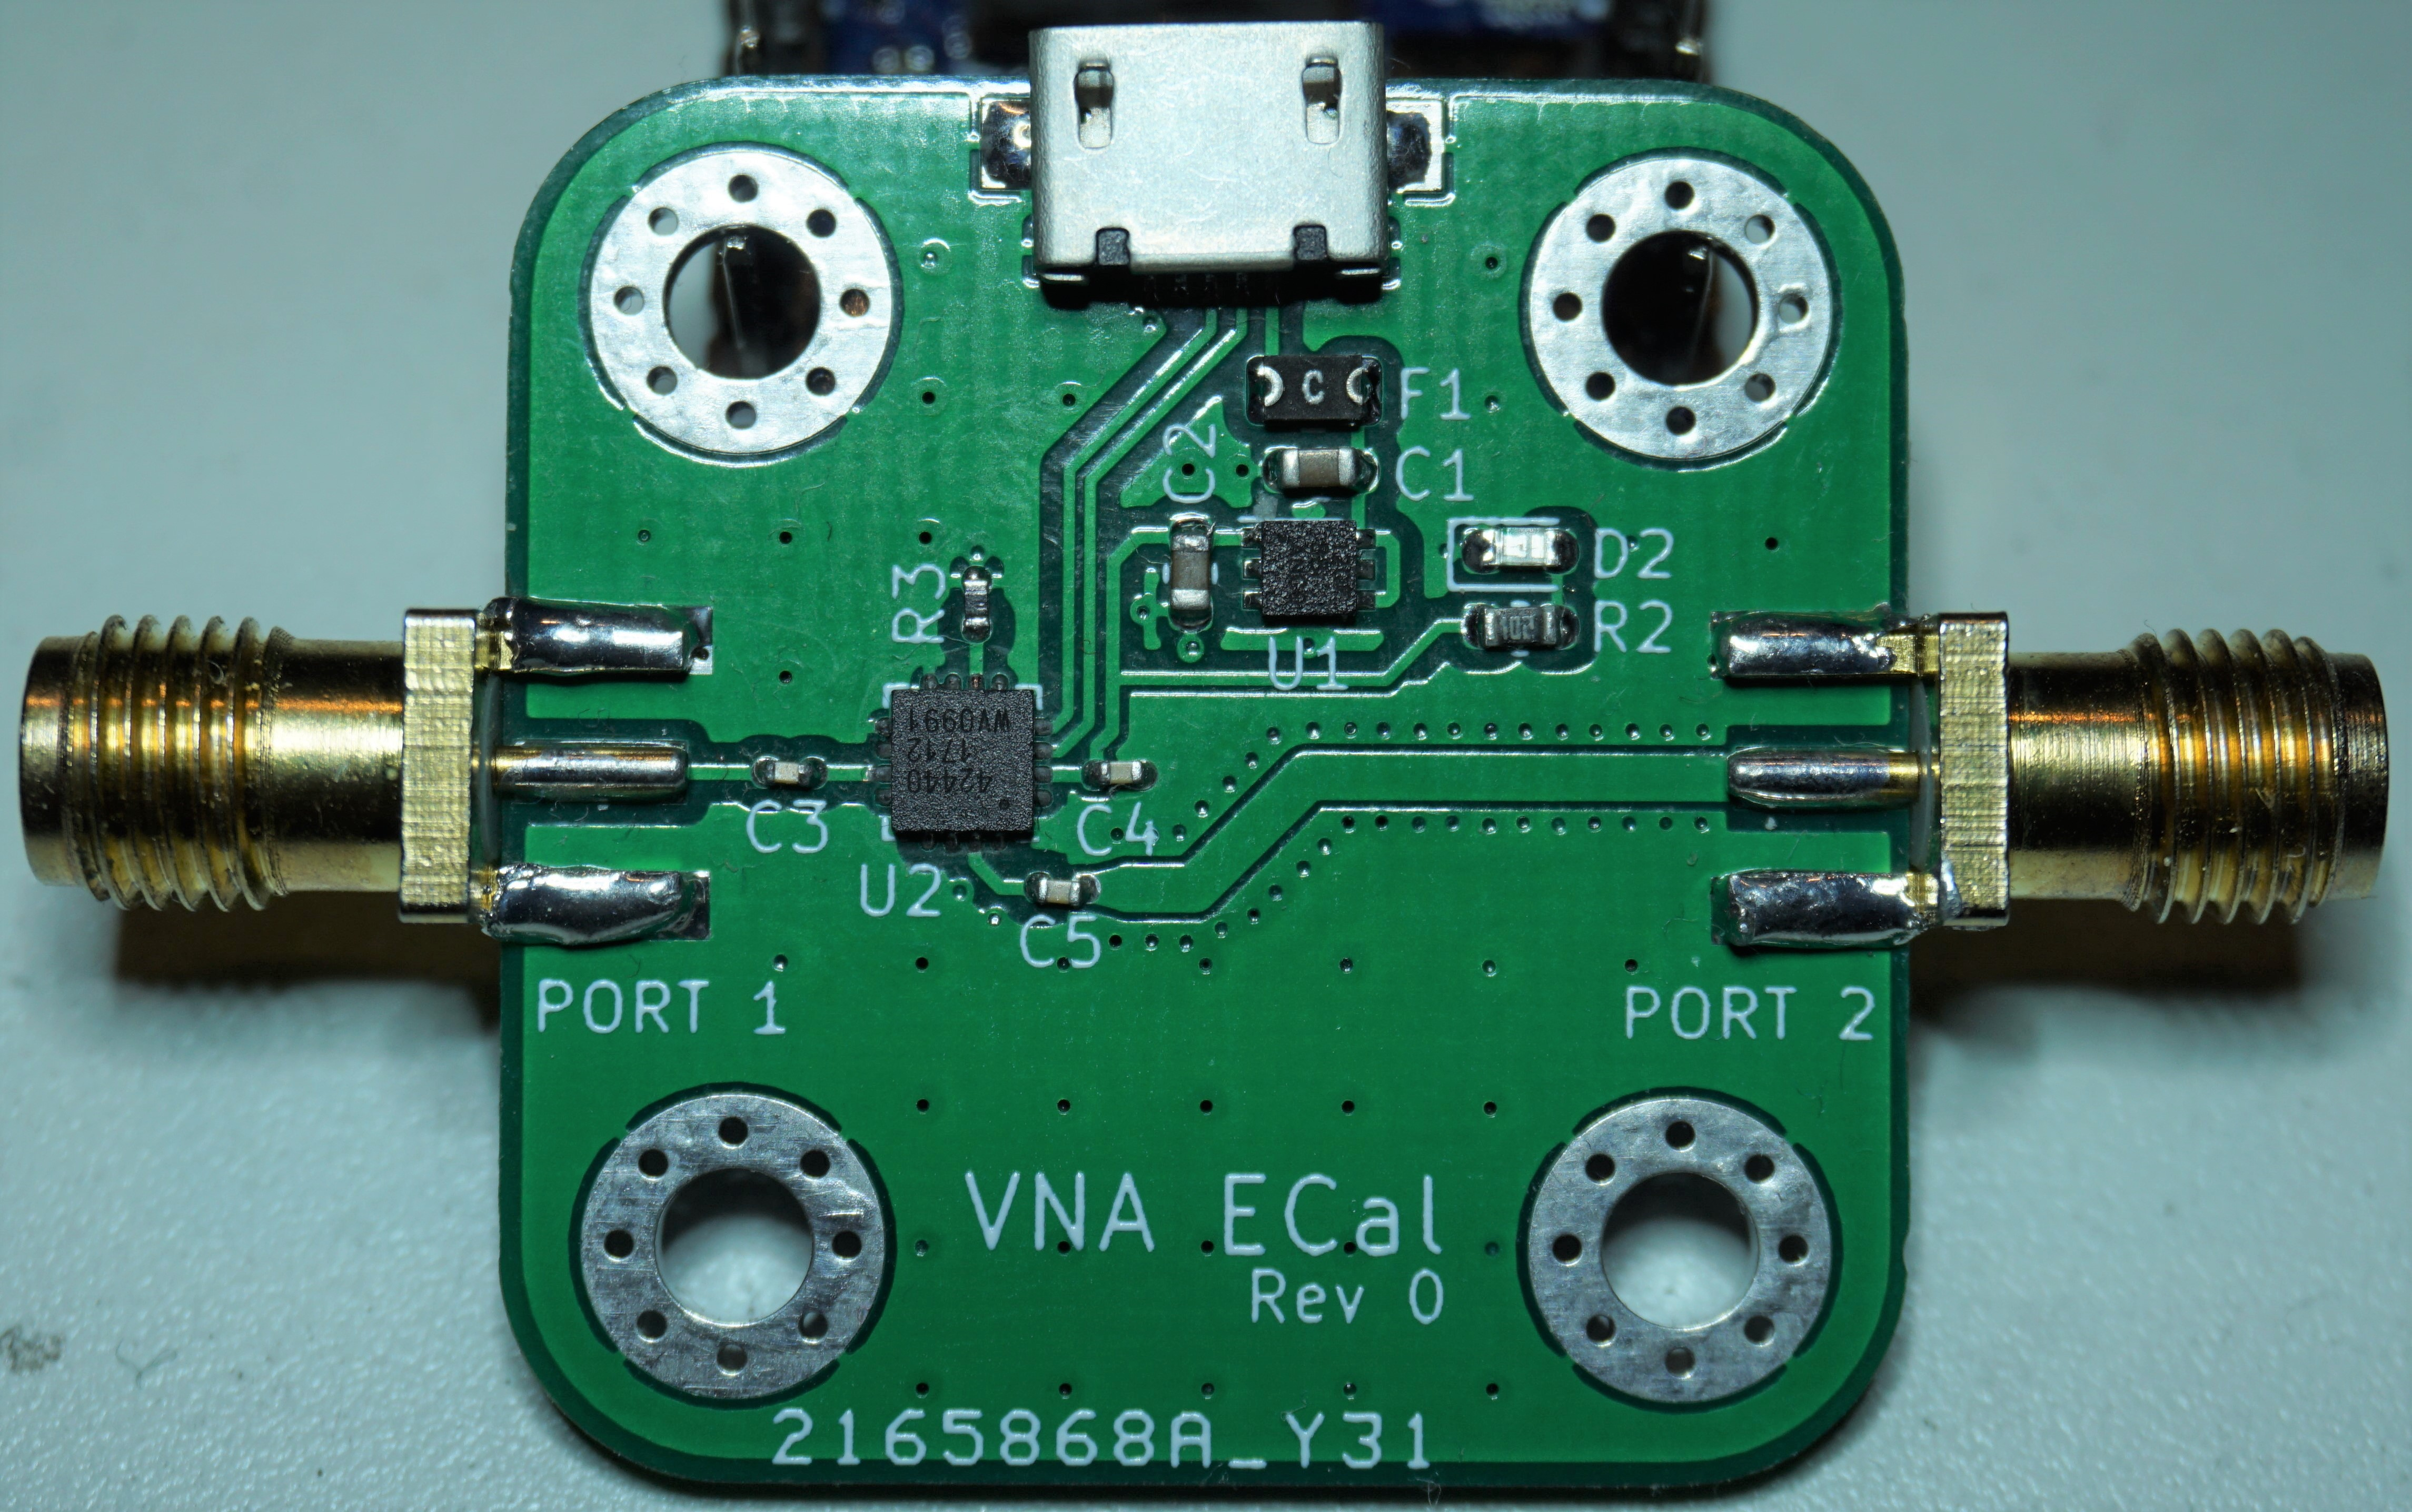
\includegraphics[width=0.65\linewidth]{ecal_board.jpg}
	\caption{Image of the ECal Unit}
	\label{fig:ecal_photo}
\end{figure}

\subsection{Firmware Development}
Firmware development for the STM32F373 was done in C, with the use of ST's Hardware Abstraction Library (HAL) configured through STM32CubeMX which allowed easy configuration and interaction with the onboard peripherals. An Eclipse based IDE, along with numerous programmers / debuggers were used for development and debugging of the firmware, which was complied with GCC to meet the requirement for an open source toolchain. As outlined in Figure \ref{fig:sw_flowchart}, there are numerous steps required to receive, process, command, measure, and return the required information for function of the VNA, and the firmware blocks developed for each of these steps will be discussed below, along with some of the challenges overcome during development. 

\subsubsection{Start-up and Initialisation}
Upon start-up, initialisation of a number of peripherals is required. Along with configuring the GPIO, SPI, timer, and USB peripherals, the ADC is initialised and calibrated, which results in reducing the offset and gain errors through an internal alignment process \cite{st_sdadc}. The pull-up on USB D+ is also cycled, as this forces re-enumeration of the device if the VNA had underdone a warm reset. 

\subsubsection{USB and Command Parsing}
A virtual COM port is used for communicating with the host computer, as due to the low data rates required and the universal compatibility of a COM port it is well suited to the task. ST's HAL provides a function which is called from an interrupt every time a character is received, however the implementation of code which handles the received data is left to the user. As such, a circular buffer was implemented which allows for receiving data, along with error checking and warnings to be sent over serial and indicated on the onboard status LED if the buffer becomes overrun or an unexpected error occurs. A function \texttt{scanUSB} was implemented to wait for a completed transmission from the VCOM port, and move the received characters into a null terminator padded string which would allow other sections of the code to parse the string without concern for it's location in the circular buffer. 

A command parser was also written which splits the received string into commands and arguments based upon defined delimiters, and then using a lookup table finds the intended function and calls it with the passed arguments. Minimal error checking is done at this stage, as it is expected that either the user or Python script which calls the function is passing correct values, and if any bad variables are passed the low level hardware control code will catch the issue. 

Along with the \texttt{measure} command which measures S-parameters, the VNA can also be commanded to act as a signal generator, sweep frequencies, configure the ECal unit, along with low level control such as configuring the output filter used, level of attenuation, enabling / disabling the PA and LO, along with reporting the status of various settings which was not only helpful during development but can be used to demonstrate the internal function for educational purposes. 

\subsubsection{Measurement Control}
When the user chooses to measure S-parameters, they pass in which parameter (S\textsubscript{11}, S\textsubscript{21}), start and stop frequency, number of steps, along with the output power level to be held throughout. From this, there are a number of steps which occur:
\begin{itemize}
	\item To indicate that the VNA is working, it illuminates a status LED blue before beginning measurement.
	\item The input switch is configured to either allow the reflected or transmitted RF to pass through to the AD8302 gain / phase detector. 
	\item The AD8302 VREF is read, as it will be used later on to remove any offset between the AD8302 and ADCs in the STM32.
	\item The required frequency step is determined, and a while loop is entered which preforms the following functions, whose workings will be described below:
	\begin{itemize}
		\item The transmit chain is configured to have the correct frequency, filters, and output power level. 
		\item The AD8302 is sampled numerous times and returns averaged voltages corresponding to the gain and phase measurements. 
		\item Conversion is then done to convert the raw voltages into gain and phase values in dB and degrees respectively, which includes the first step in phase correction. 
		\item The frequency, gain, and phase measurements are then sent over serial to the host computer, before incrementing the frequency. 
	\end{itemize}
	\item Once all required frequencies have been measured, the VNA turns its status LED green to indicate it is finished, and waits for a new command. 
\end{itemize}

\subsubsection{Transmit Chain Configuration}
Transmit chain configuration begins with the MAX2871 PLL, which was the single most challenging part of the project, as it has six 32 bit registers which all need to be configured correctly for function, however the data sheet is light on detail and I was unable to find an application note detailing configuration of it. Maxim do however provide a tool 'MAX287X' which graphically shows the user settings at each point of the internal configuration, and this in combination with the data sheet and projects found online \cite{max2871_trans} \cite{max2871_synth} enabled a Python script to be written which would match the required register values. From there, the code was ported to the STM32, and after some bit shifting to swap the endianness around the SPI transfers allowed control over the MAX2871's frequency and power. 

With respect to configuration during use, the VNA calculates the multiply and divide coefficients which need to be set to correctly multiply up the reference frequency, and in addition calculates the actual frequency the MAX2871 will output, although due to the use of a fractional-N PLL these is typically sub hertz differences between the desired and set frequencies. The VNA can also control the output power of the MAX2871 in 3dB increments, and depending on the required output power will set the output power such that the attenuator can meet the required attenuation or gain. Before configuring the MAX2871, the VNA switches in the correct filter according to a lookup table and then sends the SPI commands for the correct frequency and power settings. It then waits until the PLL has achieved lock to ensue the frequency has been set before configuring the gain. 

To set the output power, the VNA implements a loop as outlined below:
\begin{itemize}
	\item Measure output power with the AD8319 log power detector.
	\item Convert voltage to dBm at port 1.
	\item Increase / decrease attenuation at programmable attenuator by one step (0.5 dB).
	\item If within 0.5 dB break, else return to top. 
\end{itemize}
Whilst this sequence could be made much smarter by changing by the exact number of steps required, it works quite quickly and does not run often as the power output from the MAX2871 is fairly flat, and as such has been left as is. The conversion of the AD8319 voltage to dBm was originally determined by the data sheet, where the relationship between voltage and power in a 50$\Omega$ system is given by $$ V\textsubscript{out} = V\textsubscript{slope/dB} \cdot  20\log_{10}(V\textsubscript{in} / V\textsubscript{Intercept}) $$ where the slope is -22 mV / dB, and intercept is 15 dBm as per Figure 27 in the data sheet \cite{ad8319}. Due to the power detector being nominally 21 dB down from the power at port 1 as shown in the schematics, additional offset was required to compensate for this. The output power flatness was then confirmed though observing how the output power varied over frequency on a spectrum analyser, and it was seen that the VNA was within 1dB across the operating range, with the discrepancy being explained by the spectrum analyser looking at the power at the set frequency, whereas the AD8319 measures the total power, including harmonics. 

\subsubsection{AD8302 Sampling and Conversion}
With the frequency and power at port 1 set, measurement of the gain and phase measurements can occur. This is achieved by sampling the analog outputs of the AD8302, and converting them to the gain difference in dB, and phase difference in degrees respectively. 

To decrease the influence of noise and to increase the ENOB of the measurement, the analog voltage is sampled 16 times for both gain and phase, jumping between the two channels and waiting between samples in an attempt to better represent the actual signal, and pick up on the small voltage changes when the phase angle is low. These samples are then averaged, and converted to the required units. 

The gain calculation is identical to what was outlined above for the AD8319 due to the IC internals being the same, and no compensation being required for non ideal behaviour. Phase compensation on the other hand is required as the output voltage decreases as a function of frequency, and as such at higher frequencies the ideal best fit shows the phase never reaching 180$^\circ$, which is obviously not possible. The other issue with levelling off of the voltage output as the phase angle becomes small is also corrected for, and is done by proportionally 'stretching' the peaks of the phase to 180$^\circ$, ensuring that the corrected waveform always reaches 180$^\circ$ before decreasing again. The process for this was calculated using a MATLAB script then implemented in C, with the results of the correction shown in Figure \ref{fig:phase_comp}.

\begin{figure}[H]
	\centering
	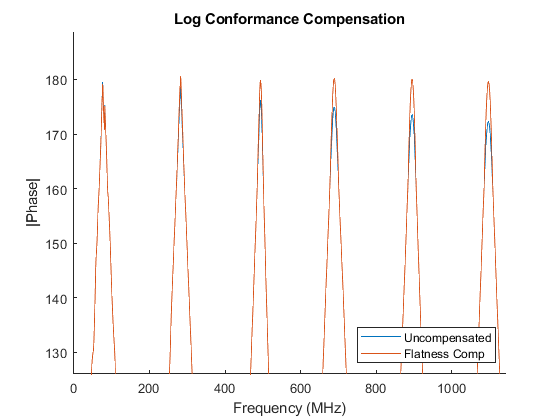
\includegraphics[width=0.8\linewidth]{log_conformance_compensation_zoomed.png}
	\caption{Correction of non idealities of the AD8302 phase detector output}
	\label{fig:phase_comp}
\end{figure}

\subsection{Software Development}

\begin{figure}[H]
	\centering
	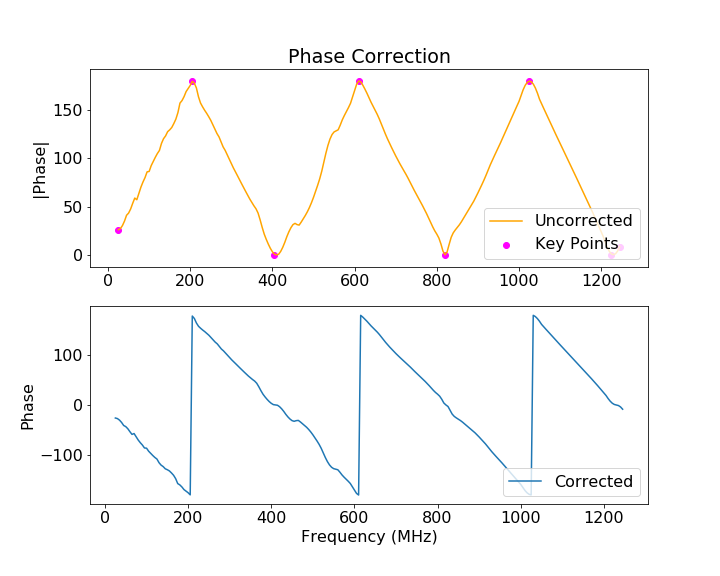
\includegraphics[width=\linewidth]{phase_correction.png}
	\caption{Absolute phase to actual phase correction}
	\label{fig:phase_correction}
\end{figure}



	\pagebreak
	
	\section{Calibration and Testing}
	\label{sec:calibration}
	\subsection{Comparison to Commercial VNAs}

Testing of the VNA consists of comparing measurements against commercial devices, and seeing how well correlated the results are. Comparisons were primarily done against an Agilent ENA Network Analyser, however due to the ENA only having a N-Type calibration kit whilst the DUTs had SMA connectors, it was unable to be used for phase measurements. For the phase measurements, a NanoVNA was utilised, which is a low cost VNA capable of functioning up to 900 MHz. Although the NanoVNA is a low cost device purchased from Ebay, it has been shown to function well enough against commercial offerings (Keysight Fieldfox) \cite{nanoVNA} that it is sufficient for use as a comparison. 

Figure \ref{fig:compare_900_s11} shows the measurement of a lumped element 900 MHz low pass filter. As can be seen, the VNA tracks fairly well, with discrepancies between the traces maximised when the magnitude ratio decreases below -20 dB, or when there is a rapid change in frequency response. The changes at lower power levels can be explained by the dynamic range of the instrument when measuring reflected power being around -25 dB.

The dynamic range of the instrument has two primary contributors: directivity of the coupler and dynamic range of the AD8302 gain and phase detector. The Mini Circuits ADC-15-4+ directional coupler utilised has between 24 and 33 dB of directivity over the frequency range of operation, which means that it is unable to differentiate any signals travelling in the forward or reverse direction below this magnitude, and as such can not identity reflected signals smaller than its dynamic range. The dynamic range of the detector is another factor, as the AD8302 can only measure differences in gain within a $\pm$30 dB range between the two RF inputs. 

As such, S\textsubscript{11} measurements will have a minimum guaranteed dynamic range of 24 dB, ranging up to 30 dB at frequencies where the dynamic range of the AD8302 becomes a limiting factor. For S\textsubscript{21} measurements which are terminated directly into the AD8302, there are no directional couplers to limit directivity and as such there is 30 dB of dynamic range. This difference in dynamic range can be seen by comparing Figures \ref{fig:compare_900_s11} and \ref{fig:compare_lfcn_s21}, where it can be seen that the dynamic range of the S\textsubscript{21} measurement in Figure \ref{fig:compare_lfcn_s21} is around 33 dB, whereas the S\textsubscript{11} measurements in Figure \ref{fig:compare_900_s11} has a maximum of approximately 27 dB. Due to corrections resulting from calibration the plotted numbers are slightly greater than theoretical, and this will be discussed later. 

With respect to the VNA not measuring the changing frequency response around 930 MHz, it is not related to the frequency response changing too quickly to be measured as there is ample time for the device to sample, however it may be a result of decreased dynamic range caused by harmonics passing from the LO to the detector, which will be discussed later with reference to Figure \ref{fig:power_unlevel}. 
\begin{figure}[H]
	\centering
	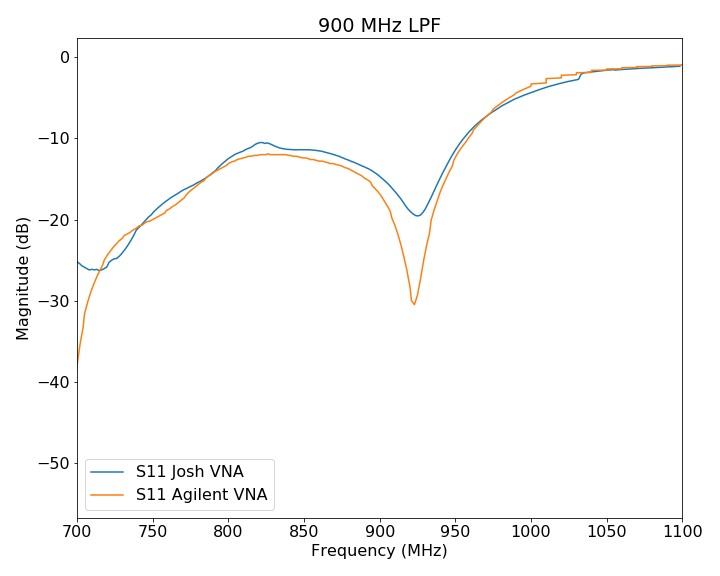
\includegraphics[width=0.8\linewidth]{900_MHz_LPF_s11.png}
	\caption{S\textsubscript{11} comparison of a 900 MHz low pass filter}
	\label{fig:compare_900_s11}
\end{figure}

Figure \ref{fig:compare_900_s21} shows an S\textsubscript{21} measurement of the same lumped element filter. There is some ripple in the passband from the VNA, along with it measuring above unity between 700 MHz and 800 MHz. This is related to the issue with LO flatness and harmonics, and will be discussed below with reference to Figure \ref{fig:power_unlevel}. The offset in frequency to the right of the commercial VNA can also be seen in Figure \ref{fig:compare_lfcn_s21}, and is most likely caused by a bug in the phase correction step, where the signal is low pass filtered which results in a lower number of elements in the set which shifts the frequency response to the left (down in frequency), and then is moved back to the correct frequencies. Given that this issue is found in both S\textsubscript{21} measurements and not S\textsubscript{11} measurements, where the phase correction algorithm does not have to deal with as many corrections due to the decreased electrical length when measuring S\textsubscript{11} directly against port 1 of the VNA, instead of through a length of coax as is required with S\textsubscript{21} measurements, it can most likely be resolved, however unfortunately there is insufficient time to explore this further. 

\begin{figure}[H]
	\centering
	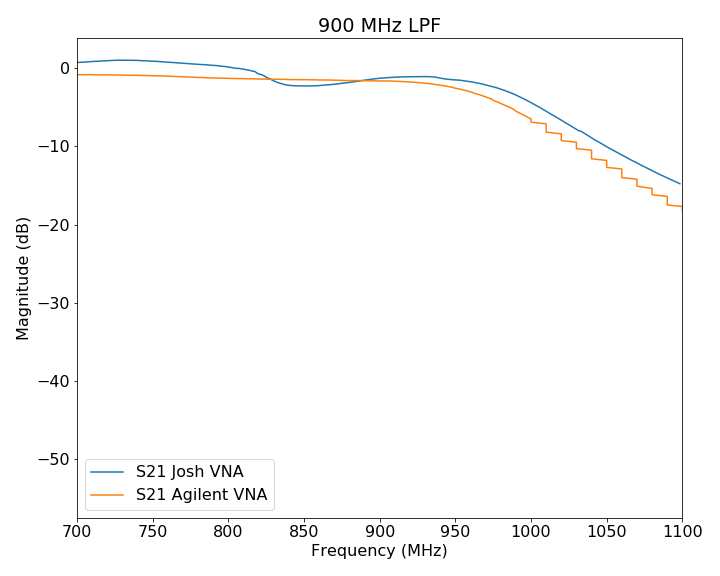
\includegraphics[width=0.8\linewidth]{900_MHz_LPF_s21.png}
	\caption{S\textsubscript{21} comparison of a 900 MHz low pass filter}
	\label{fig:compare_900_s21}
\end{figure}

Figure \ref{fig:power_unlevel} shows the power flatness from the transmit chain, and was determined by measuring S21 with both ports of the VNA terminated into 50$\Omega$ loads. Whilst this measurement would typically referred to as isolation between port 1 and 2, due to the AD8302 measuring the difference between the LO and port 2, it shows both the isolation between ports, along with the flatness of the LO in a single measurement which cannot be separated. Given both ports are terminated and the frequencies are fairly low which will result in reduced coupling between ports, it can be assumed that all of the changes in magnitude are a direct result of the power from the LO changing as a function of frequency. 

The rapid changes in power as a function of frequency are a combination of the large number of harmonics in the MAX2871 output due to it utilising a divided down output below 3 GHz, and as such the output waveform is a square wave which has numerous harmonics at integer multiples of the fundamental, along with poor filter choices to remove the harmonics, as described in \S \ref{subsubsec:lo filtering}. At the time of design it was not known that the output of the MAX2871 (and other low cost, single chip PLLs) were divided down to increase their frequency range, as it was not specified in the documentation and there was no prior experience with the IC. This resulted in the assumption that significant filtering would not be required, as any harmonics would be a significant number of dB down from the fundamental and would not impact the measurement significantly. During bring-up of the transmit chain it was connected to a spectrum analyser and the large number of harmonics was noticed, as previously measurements were done with a low bandwidth (50 MHz) oscilloscope which was unable to capture past the first harmonic and as such appeared to be less of an issue. It should be noted that the measurements done on the oscilloscope were made during bring-up of the MAX2871 and associated firmware, and were aimed to capture if there was an output and if so what was the frequency as this was a major challenge during development, and was not aimed to assess the signal quality of the output waveform due to the lack of bandwidth which would limit the representation of the signal. 

\begin{figure}[H]
	\centering
	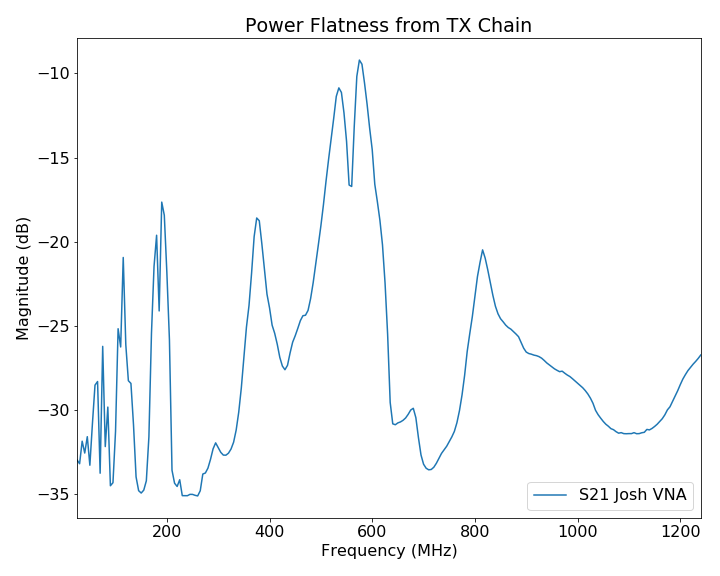
\includegraphics[width=0.8\linewidth]{power_unlevel.png}
	\caption{Power flatness from TX chain, measurements shown S\textsubscript{21} with both ports terminated into 50$\Omega$}
	\label{fig:power_unlevel}
\end{figure}

This behaviour shows itself in two main effects: ripple in the magnitude response and decreased dynamic range. The issue with ripple is most easily seen in Figure \ref{fig:compare_lfcn_s21}, where there is a noticeable peak at 550 - 600 MHz, which corresponds with the spike in power shown in Figure \ref{fig:power_unlevel}. With respect to dynamic range, it can be seen that when there is an increased reference waveform such as at 900 - 950 MHz, the measured response at that frequency (such as shown in Figure \ref{fig:compare_900_s11}) is not as low as should be. This occurs for the same reason as above, as the increased reference power increases the measured result, which presents itself as an increased noise floor.  

There are two primary methods which could be used to resolve this issue: changing the number and cut-off frequency of the filters, and changing to a superheterodyne architecture. Increasing the number of filters would allow for sufficient attenuation of harmonics across the frequency band, however going above four filters is impracticable due to the availability of switches with more than four ports, along with the significant amount of space filter banks take up. To improve performance whilst only utilising four filters, the frequency range of the VNA would need to be reduced, which is undesirable. In saying this, changing the filters would be the easiest option as it could be done to the currently assembled board with some flux and a hot air gun. 

Altering the architecture of the VNA to a superheterodyne device where the inputs to the AD8302 are downconverted to a fixed frequency would also resolve this issue, as a single filter could be used at the inputs of the receiver to filter out any unwanted frequencies as they would be downconverted to outside the bandwidth of the filter. Whilst this method would add an additional MAX2871 and two mixers to the BOM, filtering on the transmit chain could be removed which would save cost, along with allowing the VNA to function up to 6 GHz if the directional couplers are replaced during redesign of the PCB. This would however be a significant investment from a time and resource perspective, and a redesign of this nature should only be attempted if all other aspects of the VNA are shown to be working nominally to reduce the risk of having the redesign not function as desired. 

Figure \ref{fig:compare_lfcn_s21} shows the insertion loss of a 400 MHz filter from Mini Circuits (LFCN-400+) which due to it's internal construction as a multiple order device has a sharp roll off and significant (> 50 dB) attenuation in the stop band. The VNA exhibits frequency shifting and ripple in the passband as discussed above, and in addition does not have the dynamic range below 30 dB to show the full response of the filter. It does however roughly track the frequency response of the device even though it is unable to measure below 30 dB, and as such may be used for indicative measurements if a VNA or other test gear cannot be sourced to determine the exact frequency response. 
\begin{figure}[H]
	\centering
	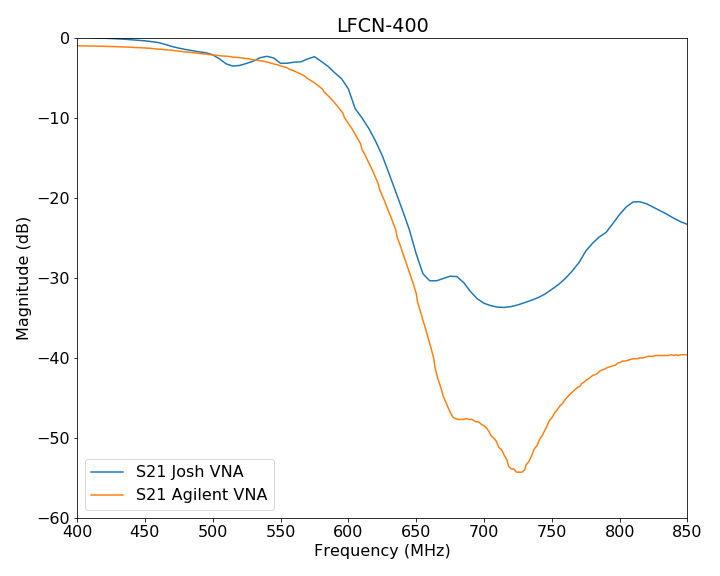
\includegraphics[width=0.8\linewidth]{LFCN-400-s21.png}
	\caption{S\textsubscript{21} comparison of a LFCN-400+ low pass filter}
	\label{fig:compare_lfcn_s21}
\end{figure}

Looking at a Smith Chart representation of the LFCN-400+ filter in Figure \ref{fig:compare_lfcn_smith}, it can be seen that there are issues with the phase measurements. Whilst the trace generally follows the expected path, it appears to have incorrect phase values in the center of the chart, where it's location relative to 50$\Omega$ is flipped, along with the path it takes until halfway between the center and edge of the chart. The large spike at 11 o'clock is a result of the dip at 500 - 550 MHz in Figure \ref{fig:compare_lfcn_s21} and is a separate issue to the phase measurement. 

This behaviour has been seen on numerous measurements, and typically occurs whenever there is a rapid change in frequency response, such as the roll off of a filter, or resonant frequency of an antenna. Whilst the cause of this is uncertain, the strange phase response can be seen from the raw AD8302 samples, and is only slightly improved when correction is applied from the calibration process. This is a problem where utilising an evaluation board with control over the amplitude and phase difference of the two input signals would be ideal, as the causal reasoning behind the undesirable output could be found, or it may not occur and then issues in other areas of the board could be investigated. In an attempt to resolve this, an AD8302 development board along with dual signal generators were acquired to allow investigation, however due to a lack of time this was unable to be attempted and as such the cause remains unknown. 

\begin{figure}[H]
	\centering
	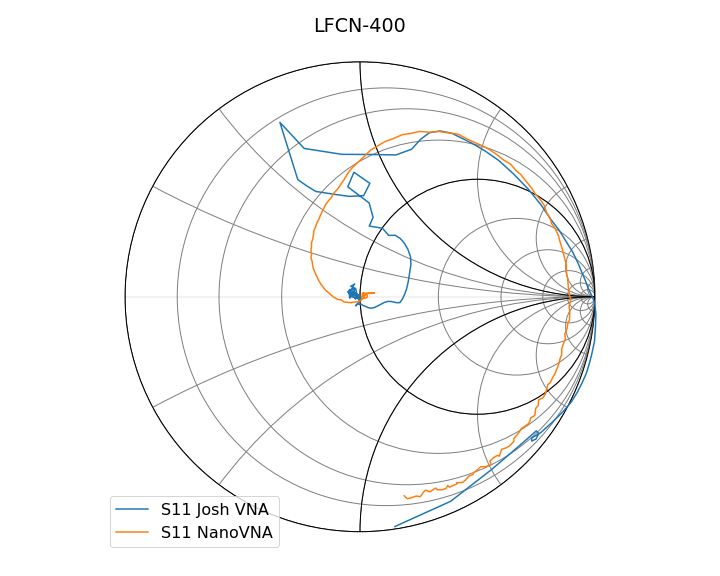
\includegraphics[width=0.8\linewidth]{LFCN-400-smith.png}
	\caption{S\textsubscript{11} comparison of a LFCN-400+ low pass filter}
	\label{fig:compare_lfcn_smith}
\end{figure}

\subsection{Calibration Efficacy}
One of the key performance metrics of a VNA is how well it can be calibrated, as this sets the measurement quality for any DUTs being measured. Figure \ref{fig:cal_sucks} shows a comparison between the load calibration standard, and the calibrated and uncalibrated measurements from the VNA. The calibration does a fairly good job at correcting the measurement so that it represents the load standard, however there are a few issues resulting from power flatness and dynamic range which cause issues with the calibration. 

Looking at the LF to 250 MHz range of the S\textsubscript{11} plot, it can be seen that the dynamic range of the AD8302 is unable to follow the > 60 dB of the calibration standard, and as a result the calibrated response is jumping all over the place in an attempt to compensate for the difference. This results in issues with the compensated phase values, which rapidly jump between +100$^\circ$ to -100$^\circ$, which is undesirable. Unfortunately this is an inherent issue with the architecture of the system and as such cannot be resolved through a hardware revision, however attempting to calibrate it against a load standard which has been altered to only have approximately a -25 dB match at low frequencies may possibly resolve this issue, as the calibration will no longer have to try adding dynamic range to the measured values. 

\begin{figure}[H]
	\centering
	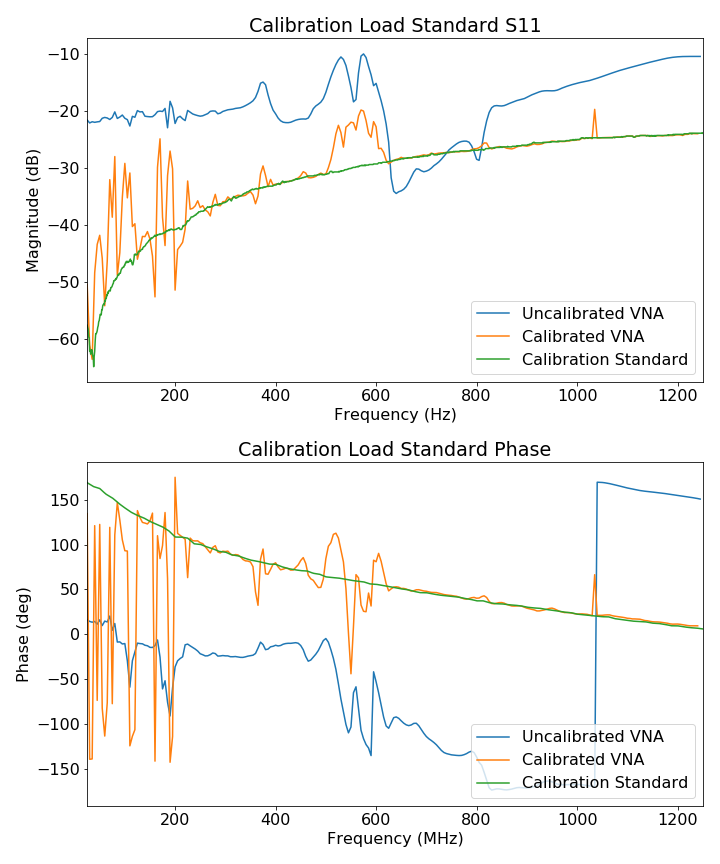
\includegraphics[width=0.8\linewidth]{load_cal_issues.png}
	\caption{S\textsubscript{11} and Phase measurements for a calibration load standard, with correction disabled and enabled.}
	\label{fig:cal_sucks}
\end{figure}

Another issue identified is the calibration not being able to compensate for large changes in power level, seen in the 500 - 600 MHz peak seen after correction. This is likely due to the twelve term calibration not accounting for LO unevenness to such a degree, and as such can not generate compensation terms to correct for the large gain in power, along with decreased dynamic range at the receiver due to the reference level increasing significantly. 

With this said, excluding the spike in magnitude at 1050 MHz due to the wrapping of phase from -180$^\circ$ to +180$^\circ$, the VNA tracks the calibration standard quite well between 600 and 1250 MHz, which suggests that if the prior two issues are rectified it may well function as expected over the whole frequency range. 

\subsection{Conclusion and Future Work}
Through research into how vector network analysers function, architecture and component selections to optimise performance of the device whilst meeting constraints, design and assembly of a RF PCBA, along with firmware and software development, a low cost VNA was designed, assembled, and tested. Due to issues with architecture and component selection there were numerous issues with the VNA which resulted in it's performance not being sufficient for the desired use cases, however the issues were identified and potential fixes suggested, which if implemented in a new revision may result in a VNA which meets the design goals. 

The key issues identified which should be looked into if future work is to be done are outlined below: 
\begin{itemize}
	\item \textbf{LO Power Flatness} needs to be resolved, with possible solutions including altering filter choices to ensure harmonics are sufficiently attenuated, altering the architecture to add a superheterodyne stage to the receiver which would result in unwanted frequencies being downconverted to outside the filter passband, or potentially selecting a new LO which has a much cleaner output spectrum.
	\item \textbf{Rectify Issues with Phase Measurements at Magnitude Transitions} is key to ensuring that the phase measurement is correct when there is a change in magnitude response, such as at a filter cut-off frequency, or at an antennas resonant frequency. 
	\item \textbf{Calibration Improvements} including resolving issues when the dynamic range of the AD8302 is insufficient to measure the DUT, along with resolving the spike in magnitude and phase when the phase wraps around on the uncorrected measurement. 
\end{itemize}
Furthermore the user experience could be improved through the addition of a graphical user interface, along with extensive documentation on how to use and modify the device, however this should only be implemented if the issues above are able to be corrected and a VNA which has sufficient accuracy is able to be implemented. 

With this said, even though the function of the VNA was not as desired there was a significant amount of insight and knowledge gained in the areas of RF design, PCB layout and assembly, along with firmware and software development which has resulted in increased technical and non technical skills which has been invaluable for professional development. 
	\pagebreak
	
	\section{References}
	\label{sec:ref}
	\printbibliography[heading=none]
	\pagebreak
	
	\section{Appendix}
	\label{sec:appendix}
	\section{VNA Design Files}
\label{appen:vna_design_files}

All files used in the design of the VNA can be found at \url{https://github.com/joshajohnson/vna}. 
Some of the files, such as the schematic, images of the PCB, and functional block diagrams are included either in the body of this thesis, or in the following pages. 

Schematics for the test boards, ECal unit, along with the code written for the VNA is not included in the thesis, as there are numerous schematics and thousands of lines of code and as such appending them would not be reasonable. The below dot points link through to the GitHub repository where some of the key files can be found if desired. 

\textbf{\href{https://github.com/joshajohnson/vna/tree/master/Hardware}{Hardware Files}}
\begin{itemize}
	\item \href{https://github.com/joshajohnson/vna/tree/master/Hardware/VNAv0}{KiCad Design Files for VNA}
	\item \href{https://github.com/joshajohnson/vna/tree/master/Hardware/VNAv0/gerbers}{VNA Gerbers}
	\item \href{https://github.com/joshajohnson/vna/tree/master/Hardware/VNAv0/renders_screenshots}{Renders and Screenshots of PCBA}
	\item \href{https://github.com/joshajohnson/vna/tree/master/Hardware/Test\%20Boards}{Functional Block Evaluation Boards}
	\item \href{https://github.com/joshajohnson/vna/tree/master/Hardware/Ecal}{ECal Hardware Design}
\end{itemize}
\textbf{\href{https://github.com/joshajohnson/vna/tree/master/Firmware/VNA}{Firmware Files} }
\begin{itemize}
	\item \href{https://github.com/joshajohnson/vna/blob/master/Firmware/VNA/Src/max2871.c}{MAX2871 Programming}
	\item
	\href{https://github.com/joshajohnson/vna/blob/master/Firmware/VNA/Src/max2871_registers.c}{MAX2871 Register Configuration}
	\item
	\href{https://github.com/joshajohnson/vna/blob/master/Firmware/VNA/Src/txChain.c}{Transmit Chain Control}
	\item
	\href{https://github.com/joshajohnson/vna/blob/master/Firmware/VNA/Src/receiver.c}{AD8302 Measurement and Initial Phase Correction}
	\item
	\href{https://github.com/joshajohnson/vna/blob/master/Firmware/VNA/Src/commandParser.c}{Command Parsing and VNA Control}
	\item \href{https://github.com/joshajohnson/vna/tree/master/Firmware/DevBoards}{Firmware Targeting Development Boards}
\end{itemize}
\textbf{\href{https://github.com/joshajohnson/vna/tree/master/Software/vna}{Software Files}}
\begin{itemize}
	\item \href{https://github.com/joshajohnson/vna/blob/master/Software/vna/vna.py}{VNA Control Software}
	\item \href{https://github.com/joshajohnson/vna/blob/master/Software/vna/phase_correction.ipynb}{Phase Correction Jupyter Notebook}
	\item \href{https://github.com/joshajohnson/vna/blob/master/Software/justTesting/ad8302Cal.m}{MATLAB Phase Compensation Script}
	\item \href{https://github.com/joshajohnson/vna/blob/master/Software/vna/calibration.ipynb}{Calibration Jupyter Notebook}
	\item \href{https://github.com/joshajohnson/vna/blob/master/Firmware/DevBoards/freqGen.py}{Python Implementation of PLL Configuration}
\end{itemize}



\begin{landscape}
	
	\begin{figure}
		\centering
		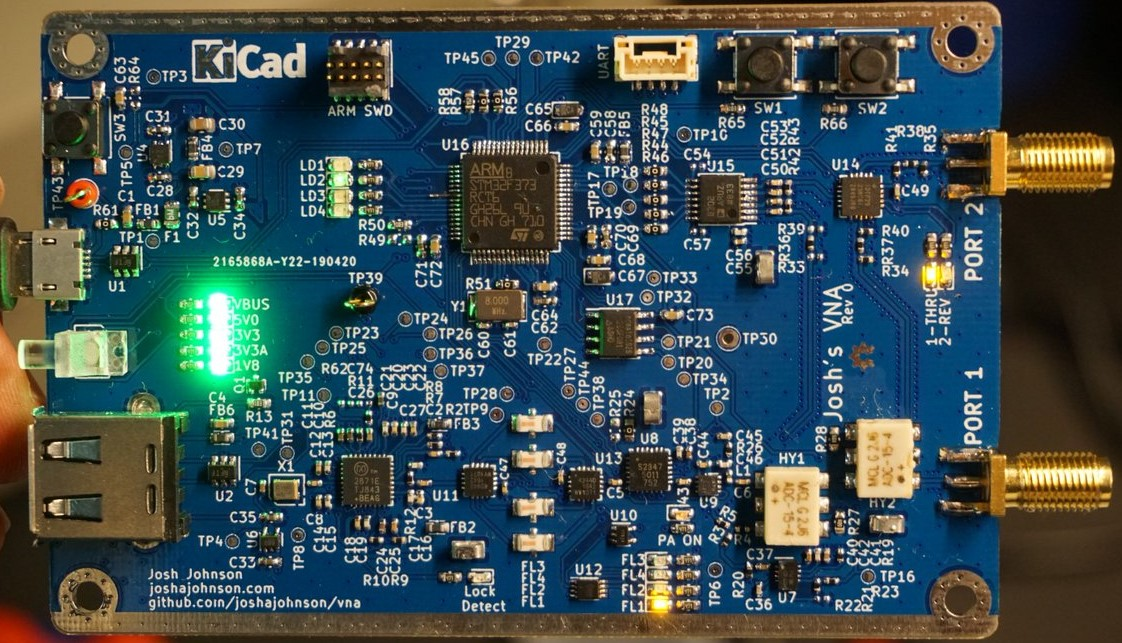
\includegraphics[width=0.9\linewidth]{vna_assembled.jpg}
		\caption{Assembled PCBA}
		\label{fig:pcb_render}
	\end{figure}

	\begin{figure}
		\centering
		\includegraphics[width=0.85\linewidth, page = 1]{vna.pdf}
		\caption{VNA Schematic - Overview}
		\label{fig:vna_schematic_overview}
	\end{figure}

	\begin{figure}
		\centering
		\includegraphics[width=0.85\linewidth, page = 2]{vna.pdf}
		\caption{VNA Schematic - LO Generation}
		\label{fig:vna_schematic_lo}
	\end{figure}
	
	\begin{figure}
		\centering
		\includegraphics[width=0.85\linewidth, page = 6]{vna.pdf}
		\caption{VNA Schematic - Filter Bank}
		\label{fig:vna_schematic_filter}
	\end{figure}
	
	\begin{figure}
		\centering
		\includegraphics[width=0.85\linewidth, page = 4]{vna.pdf}
		\caption{VNA Schematic - Source Levelling}
		\label{fig:vna_schematic_source_levelling}
	\end{figure}
	
	\begin{figure}
		\centering
		\includegraphics[width=0.85\linewidth, page = 5]{vna.pdf}
		\caption{VNA Schematic - Coupling}
		\label{fig:vna_schematic_coupling}
	\end{figure}
	
	\begin{figure}
		\centering
		\includegraphics[width=0.85\linewidth, page = 7]{vna.pdf}
		\caption{VNA Schematic - Gain and Phase Detection}
		\label{fig:vna_schematic_ad8302}
	\end{figure}
	
	\begin{figure}
		\centering
		\includegraphics[width=0.85\linewidth, page = 8]{vna.pdf}
		\caption{VNA Schematic - Microcontroller}
		\label{fig:vna_schematic_micro}
	\end{figure}
	
	\begin{figure}
		\centering
		\includegraphics[width=0.85\linewidth, page = 3]{vna.pdf}
		\caption{VNA Schematic - Power}
		\label{fig:vna_schematic_power}
	\end{figure}
\end{landscape}

\section{Board Images}
Below are a number of images which were taken during development and may of be interest, however are not directly relevant to the function of the device. 

\begin{figure}[H]
	\centering
	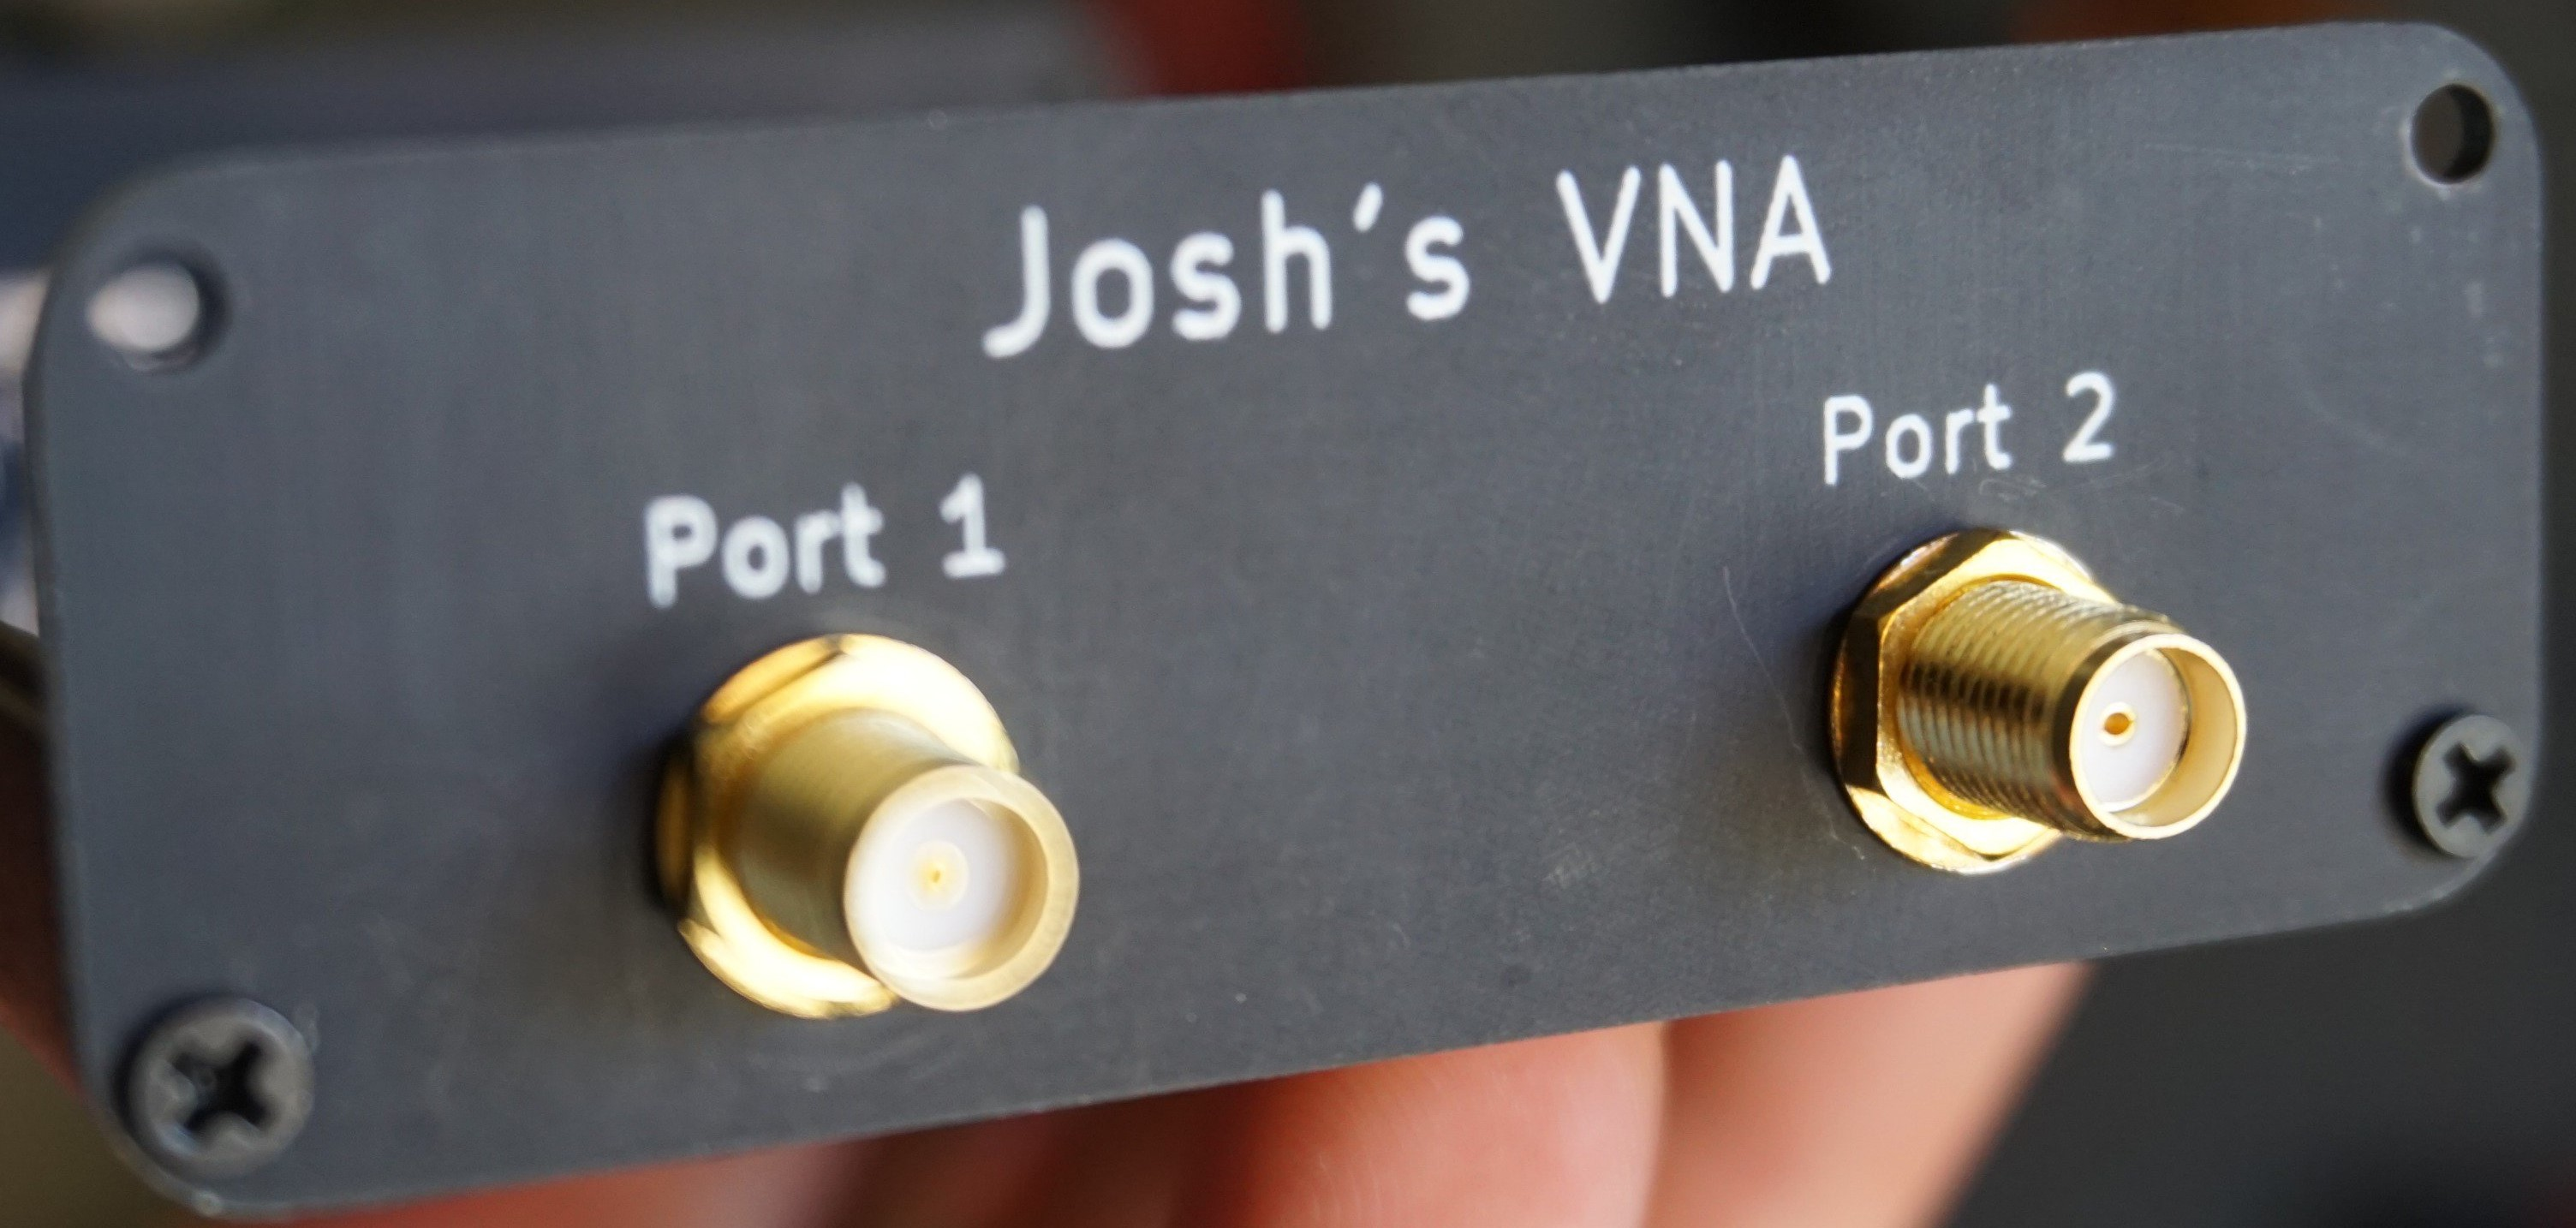
\includegraphics[width=0.8\linewidth]{vna_front_panel.jpg}
	\caption{VNA Front Panel}
	\label{fig:pcb_front_render}
\end{figure}

\begin{figure}[H]
	\centering
	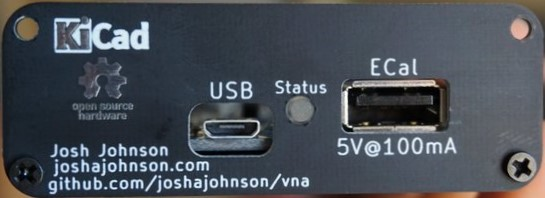
\includegraphics[width=0.85\linewidth]{vna_back_panel.jpg}
	\caption{VNA Rear Panel}
	\label{fig:pcb_rear_render}
\end{figure}

\begin{figure}[H]
	\centering
	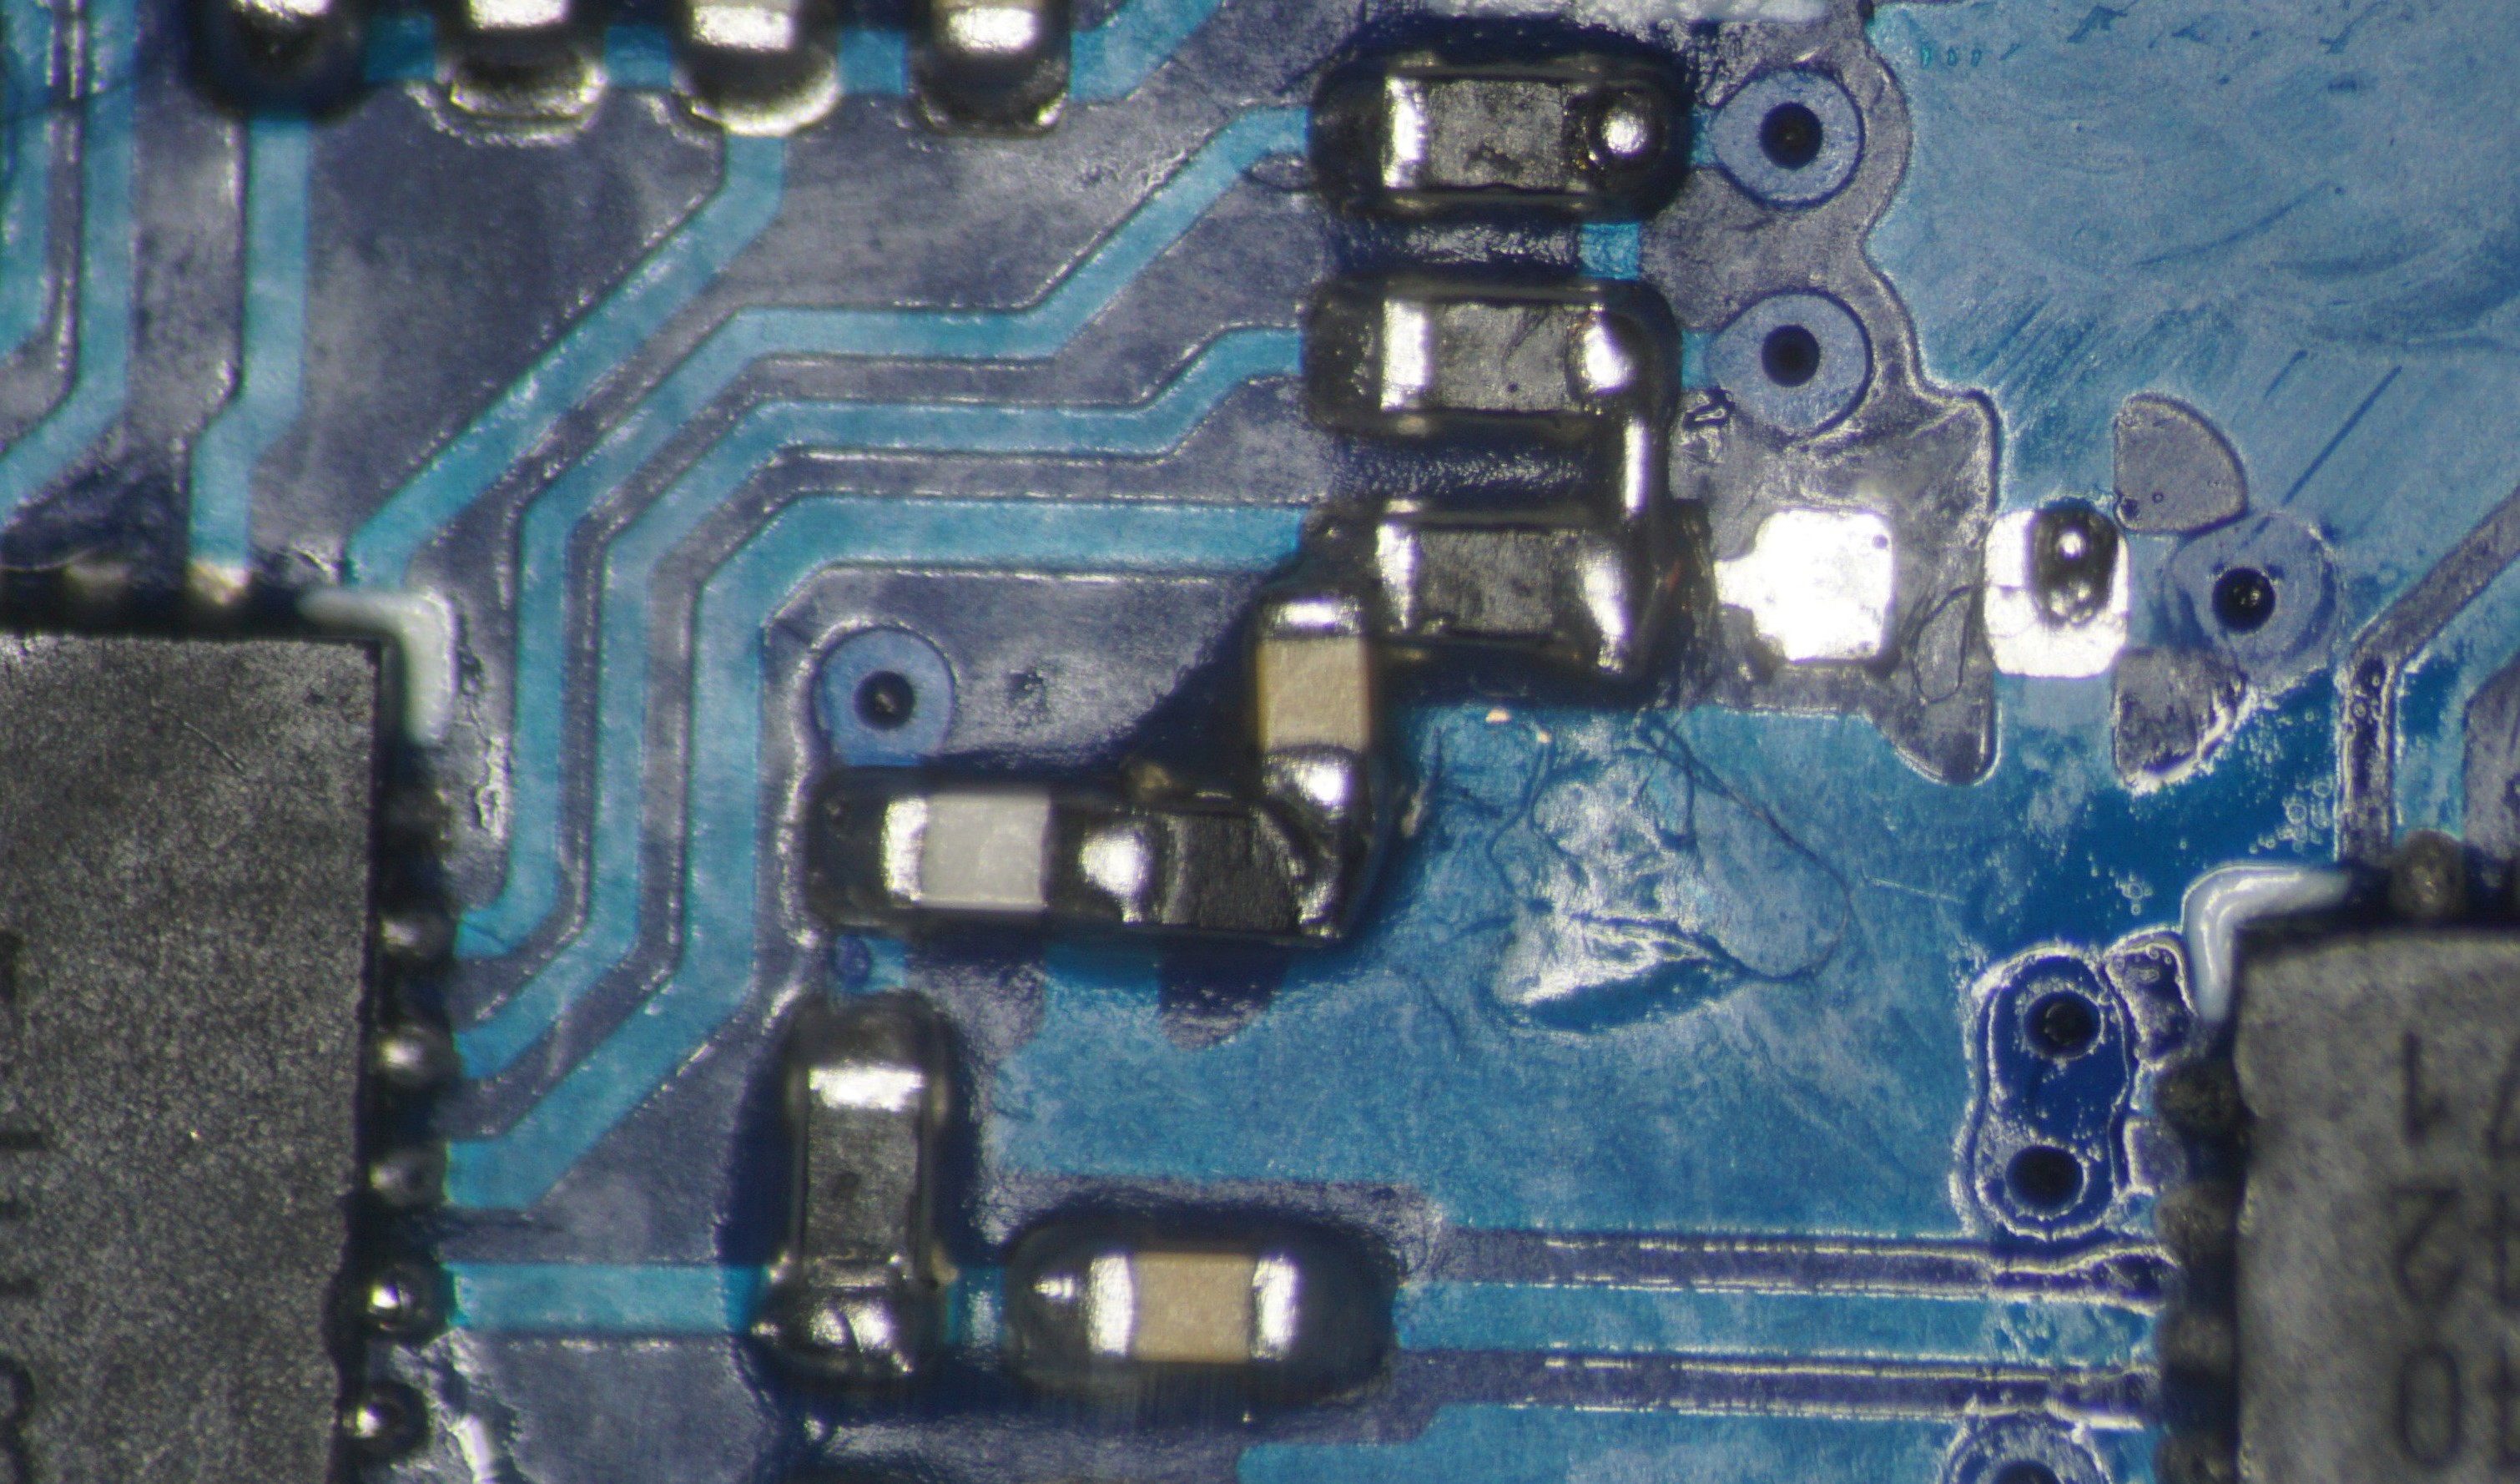
\includegraphics[width=0.7\linewidth]{max_rework.jpg}
	\caption{Rework of the MAX2871 RF- output}
	\label{fig:max_rework}
\end{figure}


\begin{figure}[H]
	\centering
	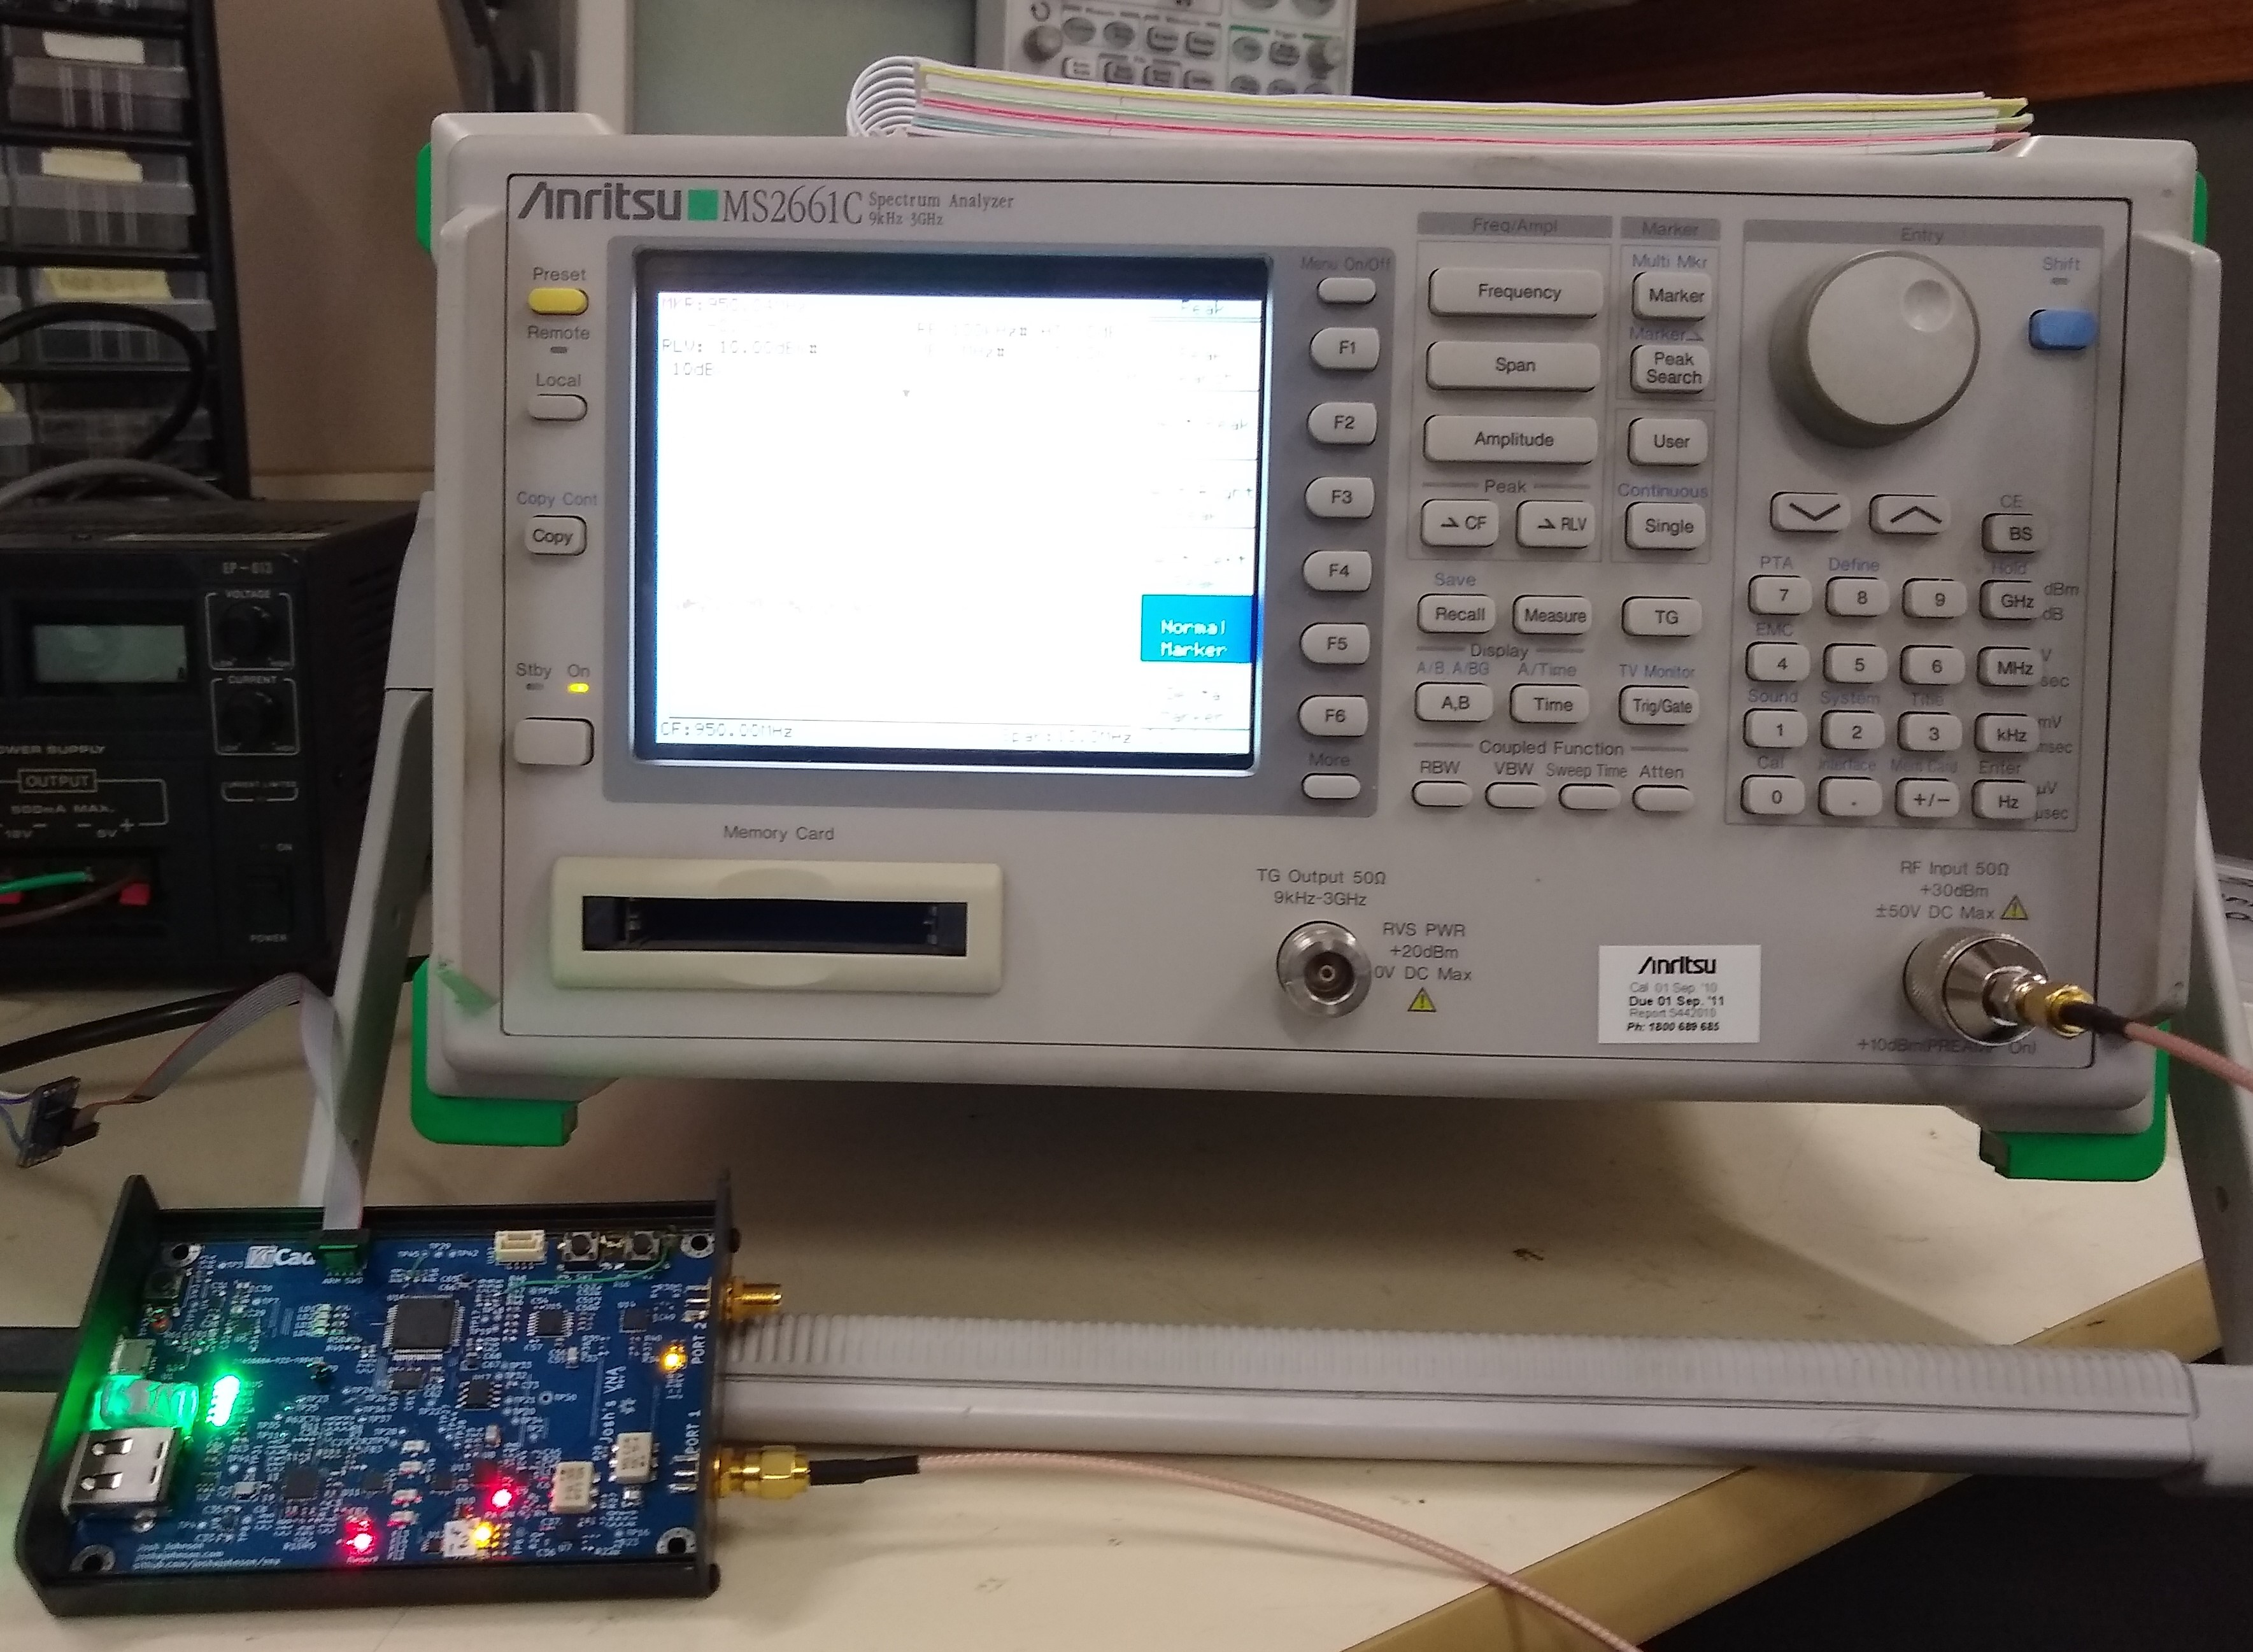
\includegraphics[width=\linewidth]{testing.jpg}
	\caption{Measurement of the output spectrum and power level control}
	\label{fig:testing_vna}
\end{figure}

\begin{figure}[H]
	\centering
	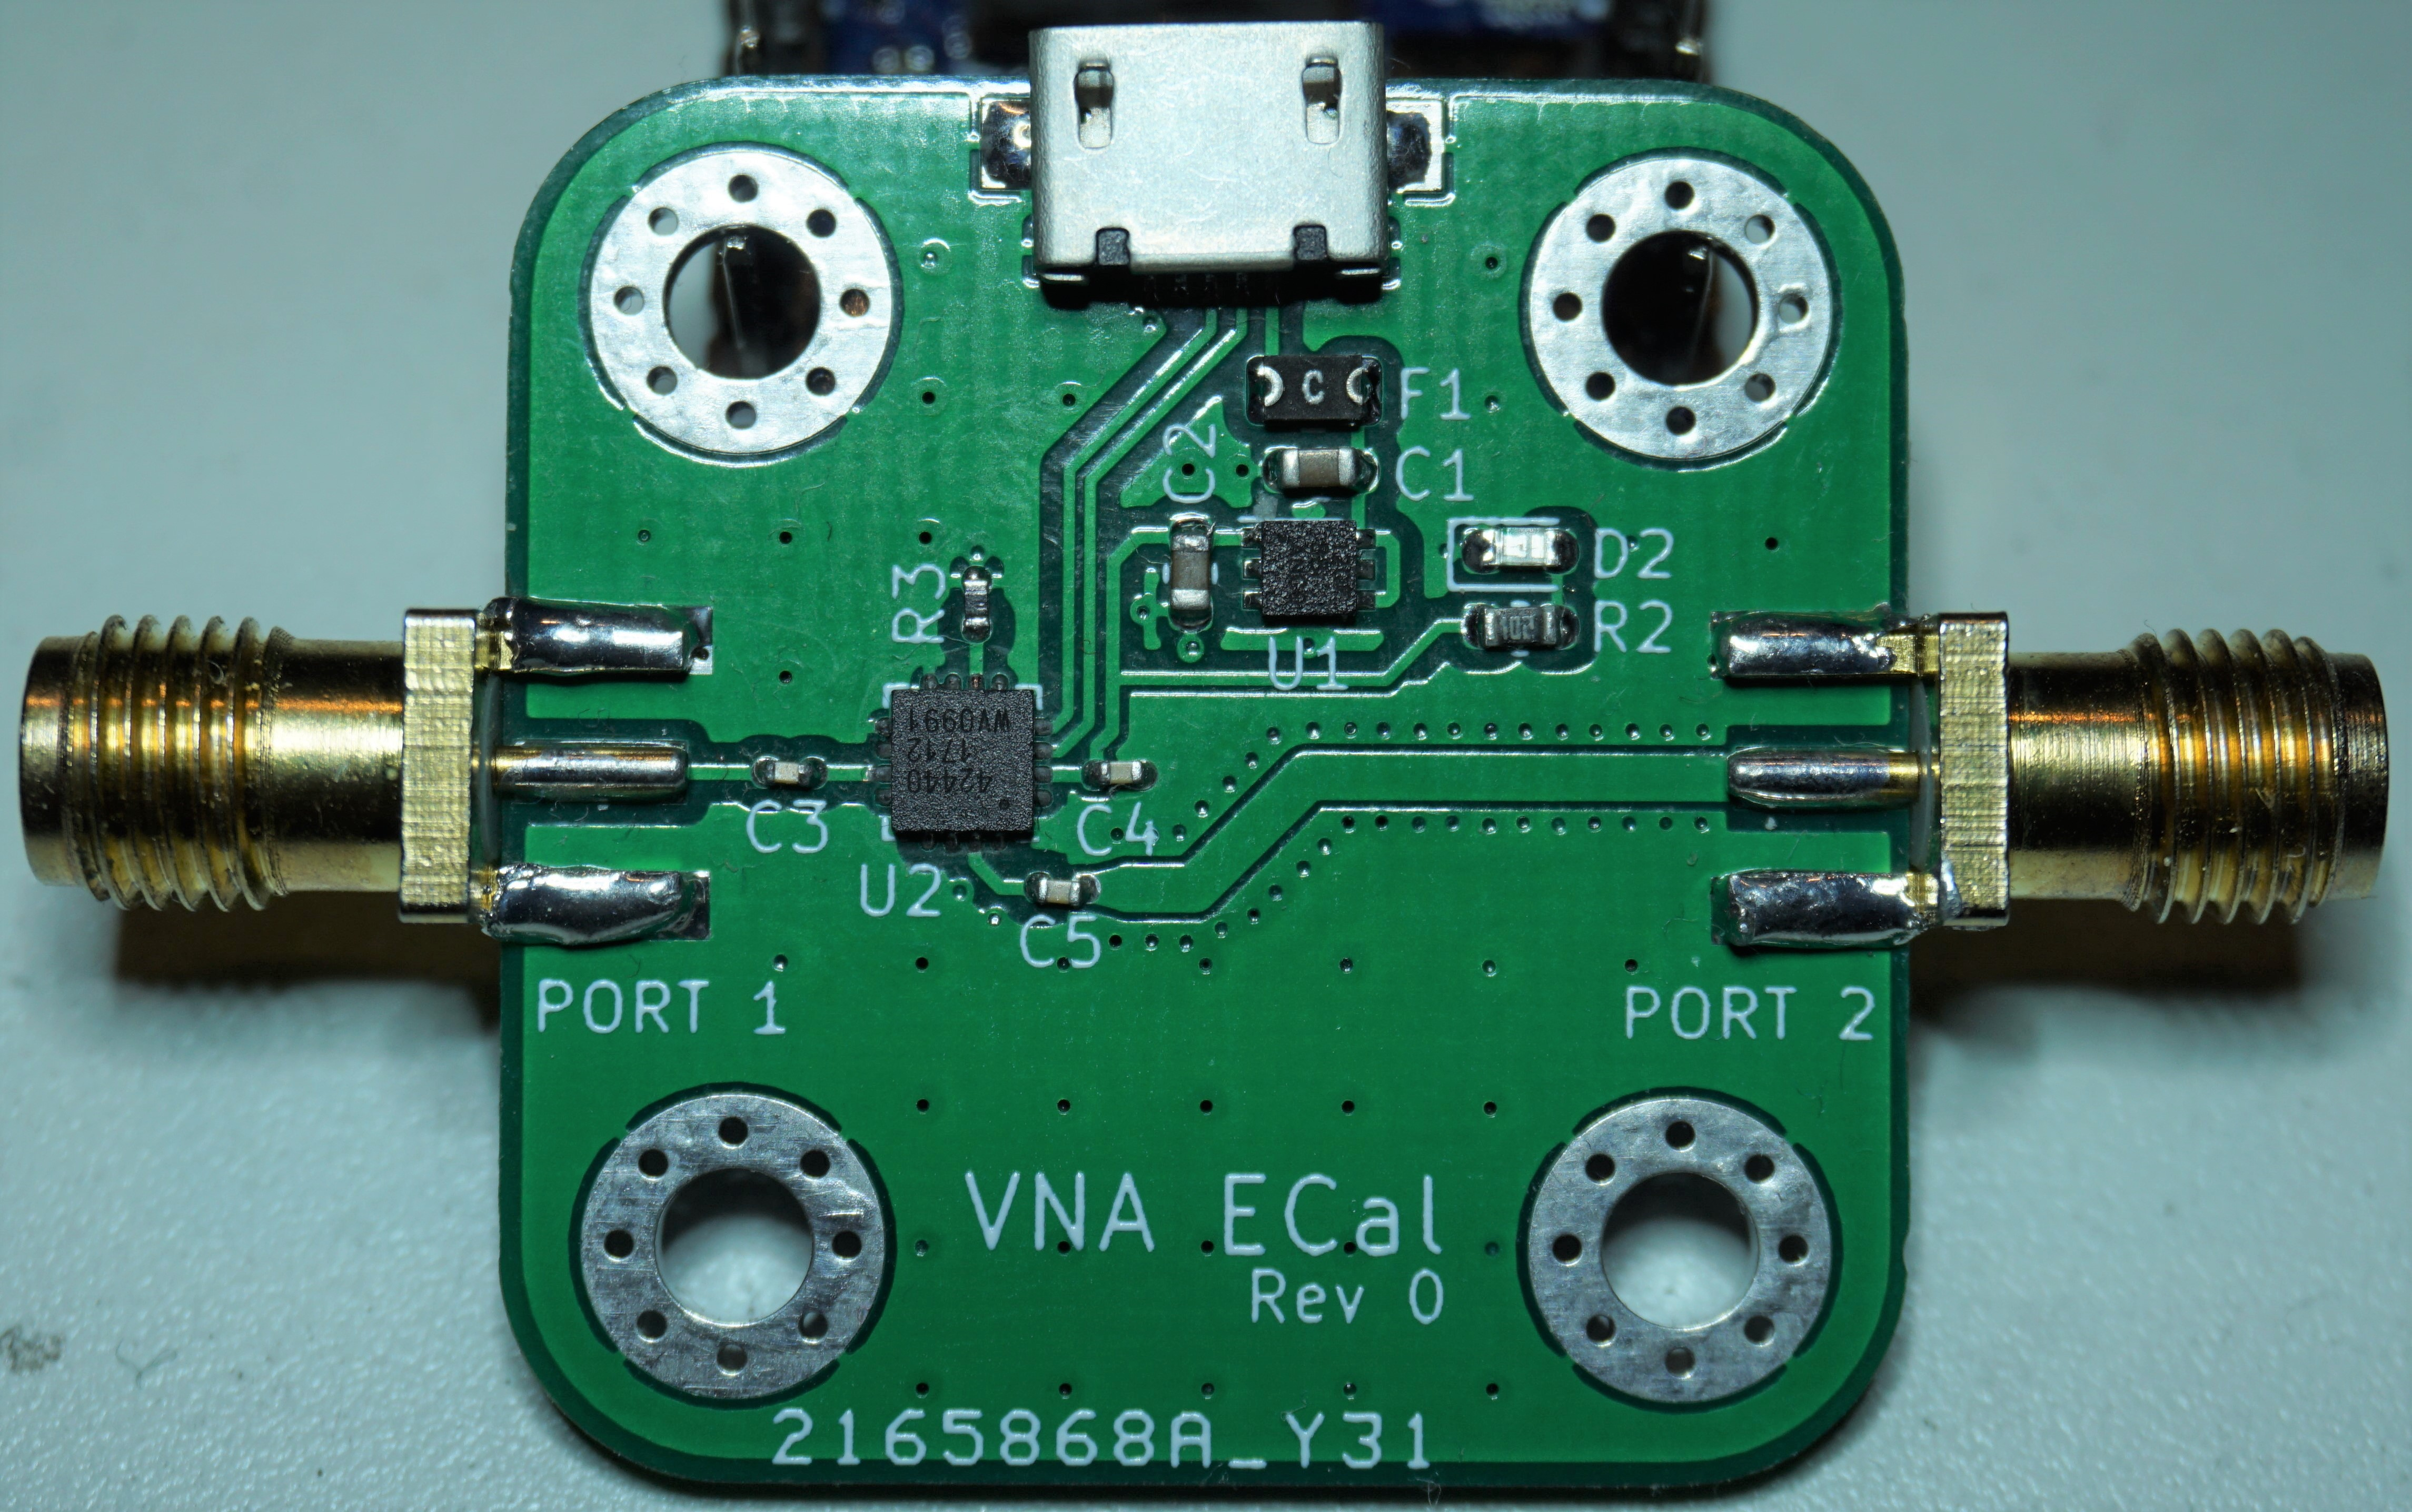
\includegraphics[width=0.9\linewidth]{ecal_board.jpg}
	\caption{Image of the ECal Unit}
	\label{fig:ecal_photo}
\end{figure}

\begin{figure}[H]
	\centering
	\includegraphics[width=0.9\linewidth]{max_dev.jpg}
	\caption{MAX2871 development board}
	\label{fig:max_dev}
\end{figure}

\begin{figure}[H]
	\centering
	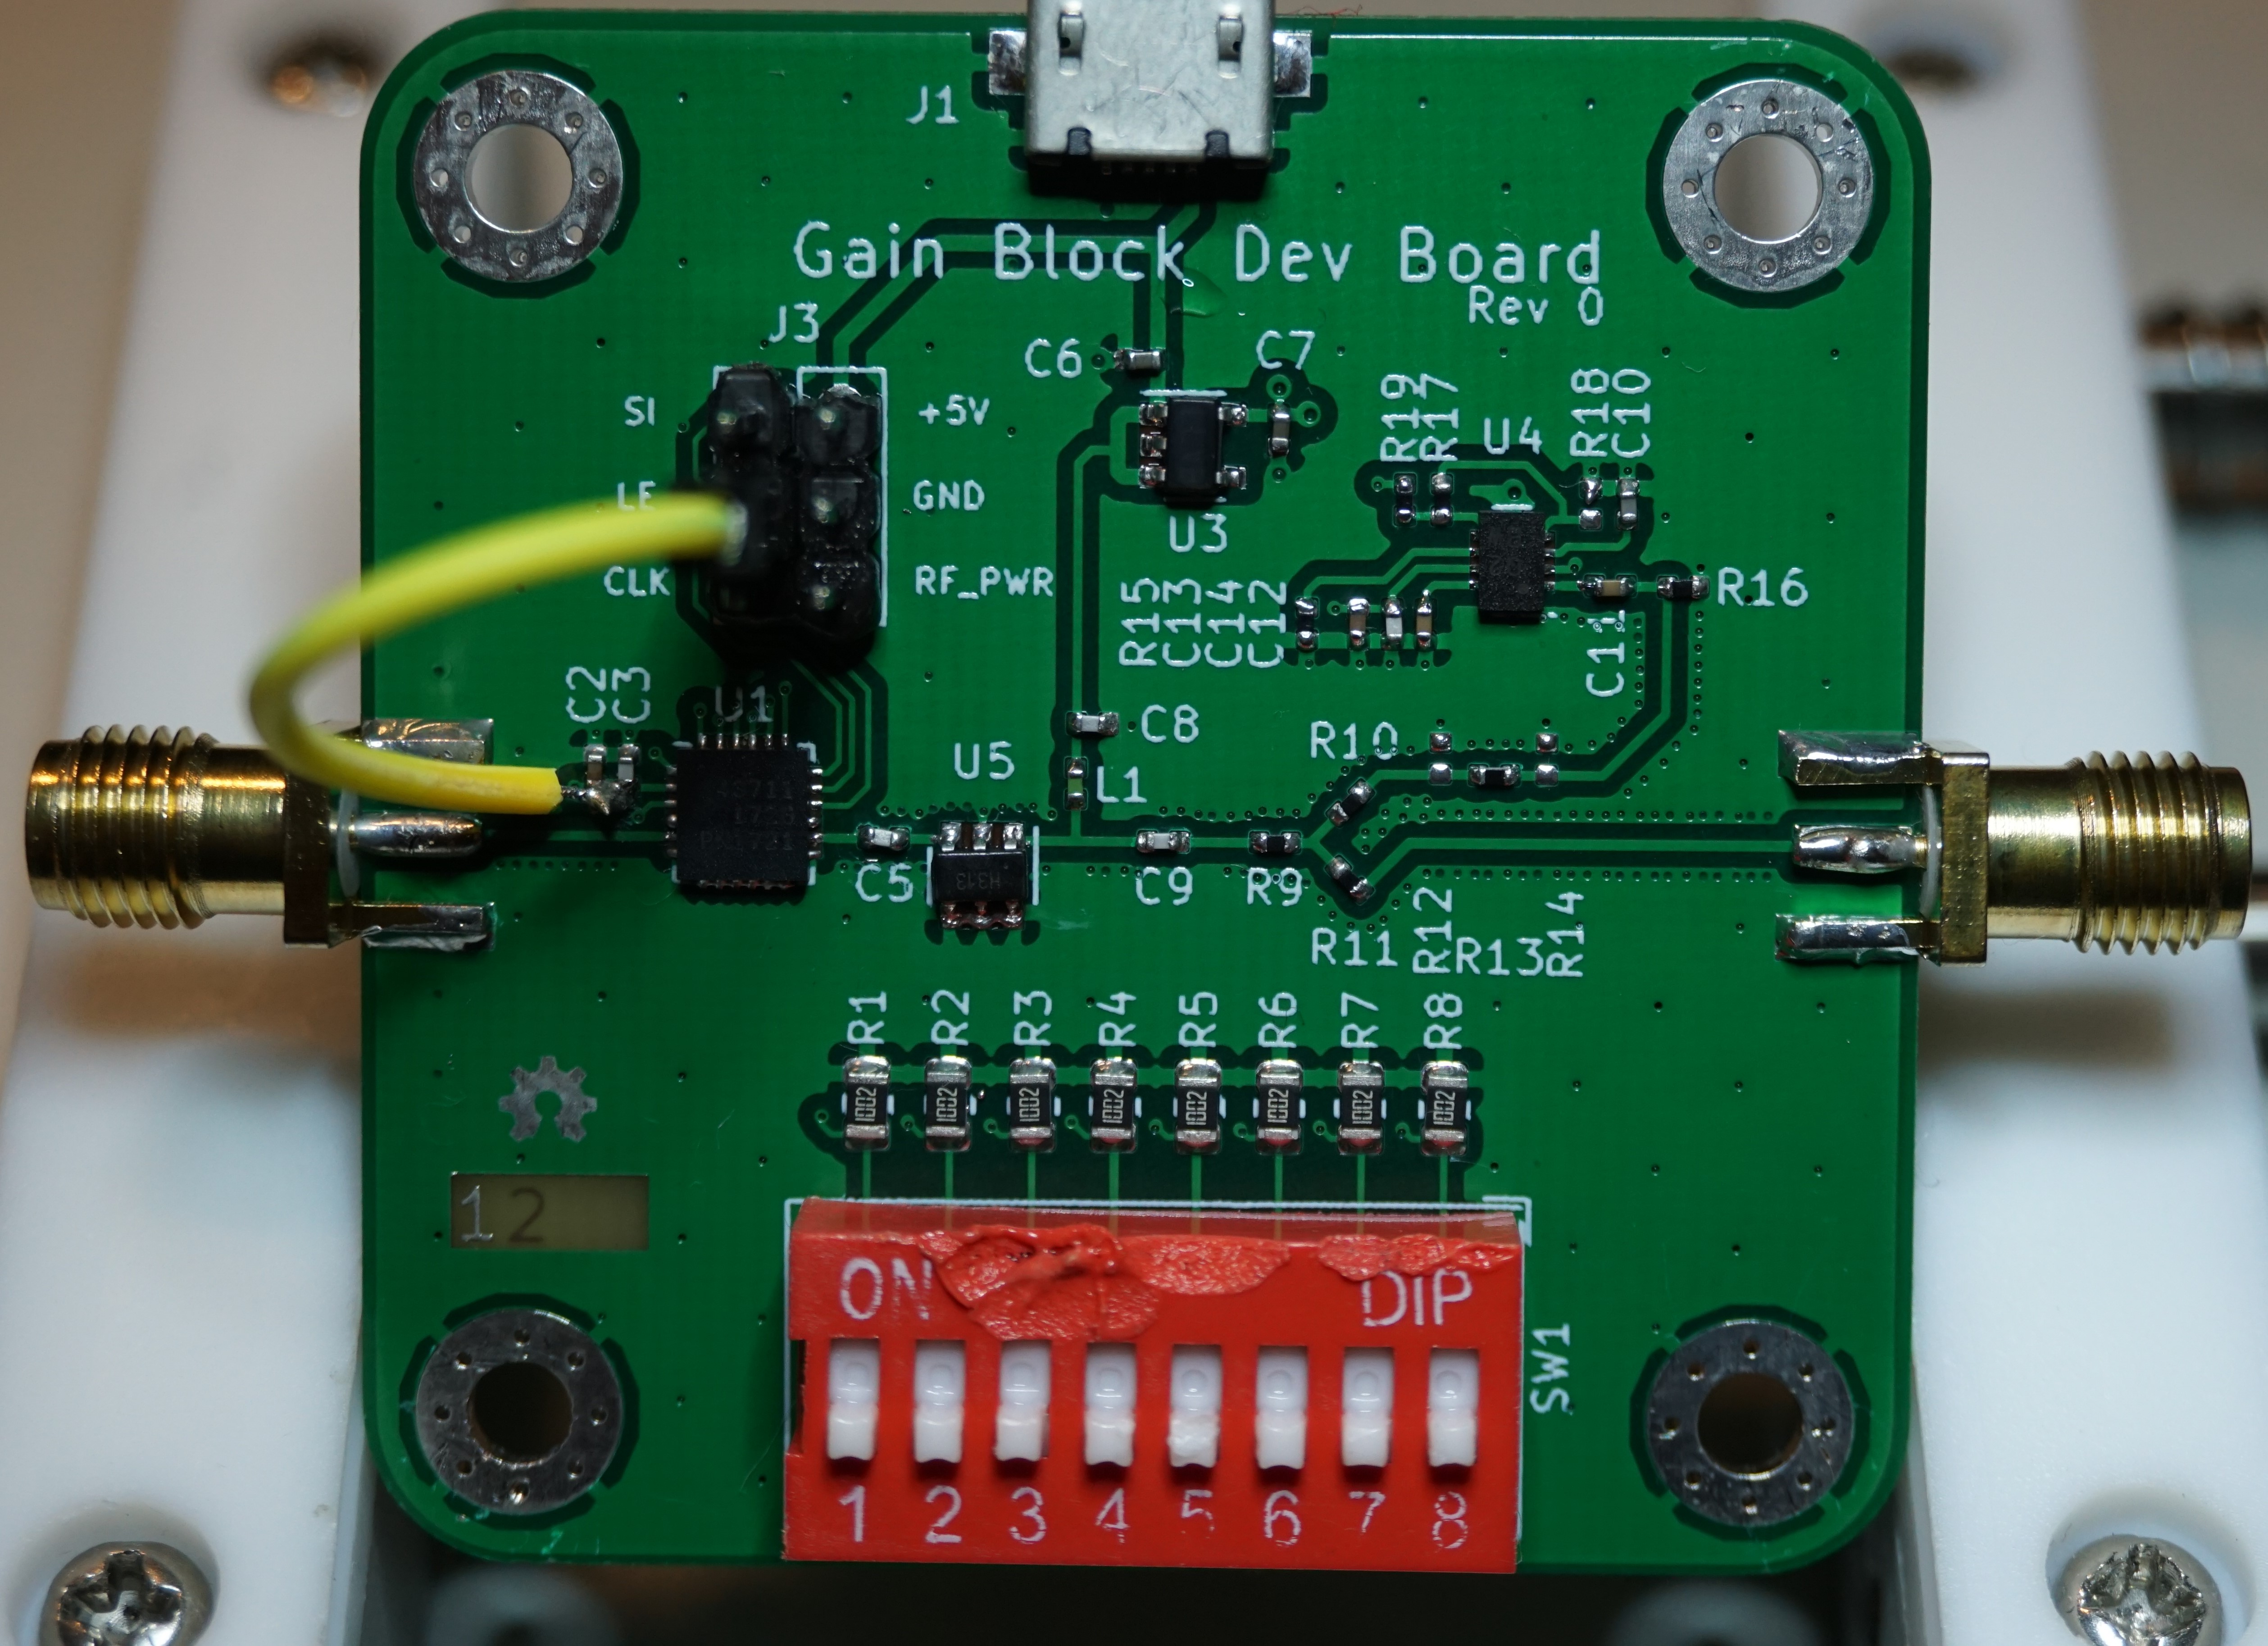
\includegraphics[width=0.9\linewidth]{level_dev.jpg}
	\caption{LO levelling development board}
	\label{fig:level_dev}
\end{figure}

\begin{figure}[H]
	\centering
	\includegraphics[width=0.9\linewidth]{coupler_dev.jpg}
	\caption{Coupler characterisation board}
	\label{fig:coulpler_dev}
\end{figure}
	
\end{document}
